% lecture1_ro.tex -- GENERATED by build_L1.py from L1_numbers.json; do not edit by hand.
\documentclass[10pt,aspectratio=169,t]{beamer}
% =============================================================================
% nn_preamble.tex -- shared Beamer preamble of Neural Networks and Deep Learning (NN)
% Used by every lecture: lectures/Lk/lecturek.tex does
%   \documentclass[10pt,aspectratio=169,t]{beamer}
%   % =============================================================================
% nn_preamble.tex -- shared Beamer preamble of Neural Networks and Deep Learning (NN)
% Used by every lecture: lectures/Lk/lecturek.tex does
%   \documentclass[10pt,aspectratio=169,t]{beamer}
%   % =============================================================================
% nn_preamble.tex -- shared Beamer preamble of Neural Networks and Deep Learning (NN)
% Used by every lecture: lectures/Lk/lecturek.tex does
%   \documentclass[10pt,aspectratio=169,t]{beamer}
%   \input{../common/nn_preamble}
%   \nnlecture{k}{Lecture title}
% Logos live in lectures/common/logos/, charts in lectures/Lk/charts/.
% Do NOT add \hfuzz / \vfuzz / \hbadness here: overfull boxes must be fixed, not hidden.
% =============================================================================

\usetheme{default}
\setbeamersize{text margin left=7mm, text margin right=7mm}

% ---------------------------------------------------------------- packages
\usepackage[utf8]{inputenc}
\usepackage[T1]{fontenc}
\usepackage{lmodern}
\usepackage{amsmath, amssymb}
\usepackage{mathtools}
\usepackage{bm}
\usepackage{tikz}
\usetikzlibrary{arrows.meta, positioning, calc, shapes.misc}
\usepackage{booktabs}
\usepackage{array}
\usepackage{graphicx}
\usepackage{colortbl}
\usepackage{xcolor}
\usepackage{multicol}
\hypersetup{colorlinks=true, linkcolor=MainBlue, urlcolor=MainBlue, citecolor=MainBlue}
\graphicspath{{../common/logos/}}   % charts are included with their language folder: charts/en/, charts/ro/

% ---------------------------------------------------------------- colours
\definecolor{MainBlue}{RGB}{26, 58, 110}
\definecolor{IDAred}{RGB}{205, 0, 0}
\definecolor{DarkGray}{RGB}{51, 51, 51}
\definecolor{FooterGray}{RGB}{100, 100, 100}
\definecolor{BlockGray}{RGB}{236, 238, 242}
\definecolor{KeynoteGray}{RGB}{218, 218, 218}
\definecolor{Crimson}{RGB}{190, 40, 50}
\definecolor{Forest}{RGB}{30, 110, 50}
\definecolor{Bitter}{RGB}{214, 150, 20}
% chart palette (same hex values and order as lectures/common/nn_plot.py SERIES)
\definecolor{Ser1}{HTML}{2A78D6}
\definecolor{Ser2}{HTML}{EB6834}
\definecolor{Ser3}{HTML}{1BAF7A}
\definecolor{Ser4}{HTML}{EDA100}
\definecolor{Ser5}{HTML}{E87BA4}
\definecolor{Ser6}{HTML}{008300}
\definecolor{Ser7}{HTML}{6250D6}
\definecolor{Ser8}{HTML}{E34948}

\setbeamertemplate{background}{%
  \begin{tikzpicture}[remember picture, overlay]
    \shade[shading=axis, shading angle=315, top color=white, bottom color=KeynoteGray]
      (current page.south west) rectangle (current page.north east);
  \end{tikzpicture}}
\setbeamercolor{background canvas}{bg=}
\setbeamercolor{structure}{fg=MainBlue}
\setbeamercolor{normal text}{fg=DarkGray}
\setbeamercolor{title}{fg=IDAred}
\setbeamercolor{frametitle}{fg=IDAred, bg=}
\setbeamercolor{block title}{bg=MainBlue, fg=white}
\setbeamercolor{block body}{bg=BlockGray, fg=DarkGray}
\setbeamercolor{block title alerted}{bg=Crimson, fg=white}
\setbeamercolor{block body alerted}{bg=Crimson!7, fg=DarkGray}
\setbeamercolor{block title example}{bg=Forest, fg=white}
\setbeamercolor{block body example}{bg=Forest!7, fg=DarkGray}
\setbeamercolor{item}{fg=MainBlue}
\setbeamerfont{frametitle}{size=\large, series=\bfseries}
\setbeamerfont{block title}{size=\small, series=\bfseries}
\setbeamertemplate{blocks}[rounded][shadow=false]
\setbeamertemplate{itemize item}{\color{MainBlue}$\boxdot$}
\setbeamertemplate{itemize subitem}{\color{MainBlue}\scriptsize$\blacktriangleright$}
% compact two-level lists: level 1 = main point, level 2 = details (no text outside bullets)
\setbeamerfont{itemize/enumerate subbody}{size=\footnotesize}
\setlength{\leftmargini}{1.1em}
\setlength{\leftmarginii}{1.1em}
\setbeamertemplate{itemize/enumerate body begin}{\setlength{\topsep}{0pt}\setlength{\partopsep}{0pt}\setlength{\parskip}{0pt}}
\setbeamertemplate{itemize/enumerate subbody begin}{\setlength{\topsep}{0pt}\setlength{\partopsep}{0pt}\setlength{\itemsep}{0pt}\vspace{-0.4ex}}

\setbeamertemplate{enumerate item}{\color{MainBlue}\insertenumlabel.}
\setlength{\leftmargini}{1.3em}
\setlength{\leftmarginii}{1.2em}
\setbeamertemplate{navigation symbols}{}
\setbeamertemplate{section in toc}{\color{MainBlue}$\blacktriangleright$~\inserttocsection}
\setbeamertemplate{caption}{\raggedright\insertcaption\par}
% frame subtitle = precise citation line under the claim title (Weron style)
\setbeamerfont{framesubtitle}{size=\footnotesize}
\setbeamercolor{framesubtitle}{fg=FooterGray}
% outline that reappears at every section with the current section highlighted
\setbeamertemplate{section in toc shaded}[default][35]
\setbeamertemplate{subsection in toc shaded}[default][35]
\setbeamertemplate{subsection in toc}{\leavevmode\leftskip=2.2em\color{DarkGray}\small\inserttocsubsection\par}
\AtBeginSection[]{{\begin{frame}{\txtoutline}\vspace{2mm}\small
  \tableofcontents[currentsection,hideothersubsections]\end{frame}}}

% ---------------------------------------------------------------- head and foot
\setbeamertemplate{headline}{%
  \vskip10pt%
  \hbox to \paperwidth{\hskip0.5cm%
    {\small\color{FooterGray}\renewcommand{\hyperlink}[2]{##2}\insertsectionhead}%
    \hfill\textcolor{FooterGray}{\small\insertframenumber}\hskip0.5cm}%
  \vskip4pt{\color{FooterGray}\hrule height 0.4pt}}
% footer as in the other courses (MFM, SFM): course name on the left, small sparkline on the right
\setbeamertemplate{footline}{%
  {\color{FooterGray}\hrule height 0.4pt}\vskip4pt%
  \hbox to \paperwidth{\hskip0.5cm%
    \textcolor{FooterGray}{\small\txtcourse}%
    \hfill\raisebox{-0.1em}{\begin{tikzpicture}[x=0.08em, y=0.08em, line width=0.4pt]
      \draw[FooterGray] (0,3) -- (1,4) -- (2,3.5) -- (3,5) -- (4,4) -- (5,6) -- (6,5.5) -- (7,4) -- (8,5) -- (9,7) -- (10,6) -- (11,5) -- (12,6.5) -- (13,8) -- (14,7) -- (15,6) -- (16,7.5) -- (17,9) -- (18,8) -- (19,7) -- (20,8.5) -- (21,10) -- (22,9) -- (23,8) -- (24,9.5);
    \end{tikzpicture}}\hskip0.5cm}%
  \vskip6pt}

% ---------------------------------------------------------------- title page
\defbeamertemplate*{title page}{nn}[1][]{%
  \vspace{0.15cm}
  \begin{center}
    \href{https://www.ase.ro}{
\includegraphics[height=0.9cm]{ase_logo.png}}\hspace{0.3cm}%
    \href{https://ipe.ro/new}{
\includegraphics[height=0.9cm]{acad_logo.png}}\hspace{0.3cm}%
    \href{https://theida.net}{
\includegraphics[height=0.9cm]{ida_logo.png}}\hspace{0.3cm}%
    \href{https://blockchain-research-center.com}{
\includegraphics[height=0.9cm]{brc_logo.png}}\hspace{0.3cm}%
    \href{https://www.ai4efin.ase.ro}{
\includegraphics[height=0.9cm]{ai4efin_logo.png}}\hspace{0.3cm}%
    \href{https://www.digital-finance-msca.com}{
\includegraphics[height=0.9cm]{msca_logo.png}}%
  \end{center}
  \vspace{0.45cm}
  \begin{center}
    \begin{minipage}{0.1\textwidth}\centering
      \href{https://quantlet.com}{
\includegraphics[height=0.9cm]{ql_logo.png}}\end{minipage}%
    \begin{minipage}{0.78\textwidth}\centering
      {\Large\bfseries\usebeamercolor[fg]{title}\inserttitle}\par\vspace{0.25cm}
      {\large\usebeamercolor[fg]{title}\insertsubtitle}\end{minipage}%
    \begin{minipage}{0.1\textwidth}\centering
      \href{https://quantinar.com}{
\includegraphics[height=0.9cm]{qr_logo.png}}\end{minipage}
  \end{center}
  \vfill
  \hspace{0.4cm}{\bfseries\insertauthor}\par\vspace{0.12cm}
  \hspace{0.4cm}\begin{minipage}[t]{0.92\textwidth}\raggedright\footnotesize\insertinstitute\end{minipage}
  \par\vspace{0.4cm}}

% ---------------------------------------------------------------- lecture metadata
\newcommand{\nnshort}{}
\newcommand{\nnnb}{notebooks}
\newcommand{\nnrepo}{https://github.com/danpele/NEURAL_BIZ/tree/main}
% language-dependent labels (English default; \nnromanian switches to Romanian, call it before \nnlecture)
\newcommand{\txtcourse}{Neural Networks and Deep Learning}
\newcommand{\txtlecture}{Lecture}
\newcommand{\txtoutline}{Outline}
\newcommand{\txtintuition}{In one sentence:}
\newcommand{\txtjob}{In practice:}
\newcommand{\txttry}{Experiment yourself:}
\newcommand{\txtwhere}{where}
\newcommand{\txtsim}{SIMULATED DATA (teaching illustration)}
\newcommand{\txtnbsuffix}{}
\newcommand{\txtinstitute}{Bucharest University of Economic Studies (ASE), Department of Statistics and Econometrics\\
    Romanian Academy, Institute for Economic Forecasting (IPE)\\
    IDA Institute Digital Assets \textbullet\ AI4EFin \textbullet\ MSCA Digital Finance}
\newcommand{\nnromanian}{%
  \renewcommand{\txtcourse}{Rețele neuronale și deep learning}%
  \renewcommand{\txtlecture}{Cursul}%
  \renewcommand{\txtoutline}{Cuprins}%
  \renewcommand{\txtintuition}{Pe scurt:}%
  \renewcommand{\txtjob}{În practică:}%
  \renewcommand{\txttry}{Exercițiu practic:}%
  \renewcommand{\txtwhere}{unde}%
  \renewcommand{\txtsim}{DATE SIMULATE (doar pentru ilustrare)}%
  \renewcommand{\txtnbsuffix}{\string_ro}%
  \renewcommand{\txtinstitute}{Academia de Studii Economice din București (ASE), Departamentul de Statistică și Econometrie\\
    Academia Română, Institutul de Prognoză Economică (IPE)\\
    IDA Institute Digital Assets \textbullet\ AI4EFin \textbullet\ MSCA Digital Finance}}
\newcommand{\nnlecture}[2]{%
  \renewcommand{\nnshort}{\txtlecture\ #1}%
  \renewcommand{\nnnb}{notebooks/L#1\string_notebook\txtnbsuffix.ipynb}%
  \title[NN]{\txtcourse}%
  \subtitle{\txtlecture\ #1: #2}%
  \author{Prof.\ dr.\ Daniel Traian PELE}%
  \institute{\txtinstitute}%
  \date{}}

% ---------------------------------------------------------------- teaching blocks (one message per frame)
% \intuition{one plain sentence}  ->  formula with every symbol defined  ->  real-data example  ->  \manager{one line}
\newcommand{\intuition}[1]{\begin{itemize}\item {\color{MainBlue}\textbf{\txtintuition}}~#1\end{itemize}\vspace{0.6mm}}
\newcommand{\manager}[1]{\colorbox{Forest!10}{\parbox{\dimexpr\linewidth-2\fboxsep\relax}{\footnotesize
  \begin{itemize}\setlength{\itemsep}{0pt}\item \textbf{\color{Forest}\txtjob}~#1\end{itemize}}}}
% Experiment yourself: pointer to the matching notebook section
\newcommand{\tryit}[1]{{\scriptsize\href{\nnrepo/\nnnb}{%
  \raisebox{-0.15em}{
\includegraphics[height=0.85em]{ql_logo.png}}\,\textbf{\txttry}~\color{MainBlue}#1}}}
% bottom row: manager line (left) + experiment pointer (right), pinned to the bottom of the frame
\newcommand{\bottomrow}[2]{\par\vfill\noindent\begin{minipage}[b]{0.72\linewidth}#1\end{minipage}\hfill
  \begin{minipage}[b]{0.26\linewidth}\raggedleft #2\end{minipage}\par\vspace{0.5mm}}
\newcommand{\where}[1]{{\footnotesize\textbf{\txtwhere}~#1\par}}

% ---------------------------------------------------------------- helpers
% chart source line under a figure: \chartsource{Source ...; period ...}
\newcommand{\chartsource}[1]{\par\vspace{1pt}{\scriptsize\color{FooterGray}#1\par}}
% link to code: \quantlet{label}{path inside the repo}
\newcommand{\quantlet}[2]{\par\vspace{1pt}\hfill\href{\nnrepo/#2}{%
  \raisebox{-0.15em}{
\includegraphics[height=0.75em]{ql_logo.png}}\textcolor{MainBlue}{\scriptsize\ #1}}}
% inline Quantlet link for the bottom-right corner of a frame: \qlink{label}{path inside the repo}
\newcommand{\qlink}[2]{{\scriptsize\href{\nnrepo/#2}{\raisebox{-0.15em}{
\includegraphics[height=0.85em]{ql_logo.png}}\,\textcolor{MainBlue}{#1}}}}
\newcommand{\simlabel}{\colorbox{Crimson!12}{\scriptsize\bfseries\color{Crimson}\txtsim}}
\newcommand{\E}{\mathbb{E}}
\newcommand{\Var}{\operatorname{Var}}
\newcommand{\Cov}{\operatorname{Cov}}
\newcommand{\Corr}{\operatorname{Corr}}
\newcommand{\asinh}{\operatorname{asinh}}
\newcommand{\iid}{\overset{\text{i.i.d.}}{\sim}}
\newcommand{\EUR}{EUR}
% deep-learning notation (Bishop & Bishop, 2024): vectors bold lower case, matrices bold upper case
\newcommand{\R}{\mathbb{R}}
\newcommand{\vx}{\mathbf{x}}
\newcommand{\vy}{\mathbf{y}}
\newcommand{\vz}{\mathbf{z}}
\newcommand{\vh}{\mathbf{h}}
\newcommand{\vw}{\mathbf{w}}
\newcommand{\vb}{\mathbf{b}}
\newcommand{\mW}{\mathbf{W}}
\newcommand{\mX}{\mathbf{X}}
\newcommand{\btheta}{\boldsymbol{\theta}}
\newcommand{\loss}{\mathcal{L}}
\newcommand{\dataset}{\mathcal{D}}
\DeclareMathOperator*{\argmin}{arg\,min}
\DeclareMathOperator*{\argmax}{arg\,max}
\DeclareMathOperator{\softmax}{softmax}
\DeclareMathOperator{\ReLU}{ReLU}
\DeclareMathOperator{\sigm}{\sigma}

%   \nnlecture{k}{Lecture title}
% Logos live in lectures/common/logos/, charts in lectures/Lk/charts/.
% Do NOT add \hfuzz / \vfuzz / \hbadness here: overfull boxes must be fixed, not hidden.
% =============================================================================

\usetheme{default}
\setbeamersize{text margin left=7mm, text margin right=7mm}

% ---------------------------------------------------------------- packages
\usepackage[utf8]{inputenc}
\usepackage[T1]{fontenc}
\usepackage{lmodern}
\usepackage{amsmath, amssymb}
\usepackage{mathtools}
\usepackage{bm}
\usepackage{tikz}
\usetikzlibrary{arrows.meta, positioning, calc, shapes.misc}
\usepackage{booktabs}
\usepackage{array}
\usepackage{graphicx}
\usepackage{colortbl}
\usepackage{xcolor}
\usepackage{multicol}
\hypersetup{colorlinks=true, linkcolor=MainBlue, urlcolor=MainBlue, citecolor=MainBlue}
\graphicspath{{../common/logos/}}   % charts are included with their language folder: charts/en/, charts/ro/

% ---------------------------------------------------------------- colours
\definecolor{MainBlue}{RGB}{26, 58, 110}
\definecolor{IDAred}{RGB}{205, 0, 0}
\definecolor{DarkGray}{RGB}{51, 51, 51}
\definecolor{FooterGray}{RGB}{100, 100, 100}
\definecolor{BlockGray}{RGB}{236, 238, 242}
\definecolor{KeynoteGray}{RGB}{218, 218, 218}
\definecolor{Crimson}{RGB}{190, 40, 50}
\definecolor{Forest}{RGB}{30, 110, 50}
\definecolor{Bitter}{RGB}{214, 150, 20}
% chart palette (same hex values and order as lectures/common/nn_plot.py SERIES)
\definecolor{Ser1}{HTML}{2A78D6}
\definecolor{Ser2}{HTML}{EB6834}
\definecolor{Ser3}{HTML}{1BAF7A}
\definecolor{Ser4}{HTML}{EDA100}
\definecolor{Ser5}{HTML}{E87BA4}
\definecolor{Ser6}{HTML}{008300}
\definecolor{Ser7}{HTML}{6250D6}
\definecolor{Ser8}{HTML}{E34948}

\setbeamertemplate{background}{%
  \begin{tikzpicture}[remember picture, overlay]
    \shade[shading=axis, shading angle=315, top color=white, bottom color=KeynoteGray]
      (current page.south west) rectangle (current page.north east);
  \end{tikzpicture}}
\setbeamercolor{background canvas}{bg=}
\setbeamercolor{structure}{fg=MainBlue}
\setbeamercolor{normal text}{fg=DarkGray}
\setbeamercolor{title}{fg=IDAred}
\setbeamercolor{frametitle}{fg=IDAred, bg=}
\setbeamercolor{block title}{bg=MainBlue, fg=white}
\setbeamercolor{block body}{bg=BlockGray, fg=DarkGray}
\setbeamercolor{block title alerted}{bg=Crimson, fg=white}
\setbeamercolor{block body alerted}{bg=Crimson!7, fg=DarkGray}
\setbeamercolor{block title example}{bg=Forest, fg=white}
\setbeamercolor{block body example}{bg=Forest!7, fg=DarkGray}
\setbeamercolor{item}{fg=MainBlue}
\setbeamerfont{frametitle}{size=\large, series=\bfseries}
\setbeamerfont{block title}{size=\small, series=\bfseries}
\setbeamertemplate{blocks}[rounded][shadow=false]
\setbeamertemplate{itemize item}{\color{MainBlue}$\boxdot$}
\setbeamertemplate{itemize subitem}{\color{MainBlue}\scriptsize$\blacktriangleright$}
% compact two-level lists: level 1 = main point, level 2 = details (no text outside bullets)
\setbeamerfont{itemize/enumerate subbody}{size=\footnotesize}
\setlength{\leftmargini}{1.1em}
\setlength{\leftmarginii}{1.1em}
\setbeamertemplate{itemize/enumerate body begin}{\setlength{\topsep}{0pt}\setlength{\partopsep}{0pt}\setlength{\parskip}{0pt}}
\setbeamertemplate{itemize/enumerate subbody begin}{\setlength{\topsep}{0pt}\setlength{\partopsep}{0pt}\setlength{\itemsep}{0pt}\vspace{-0.4ex}}

\setbeamertemplate{enumerate item}{\color{MainBlue}\insertenumlabel.}
\setlength{\leftmargini}{1.3em}
\setlength{\leftmarginii}{1.2em}
\setbeamertemplate{navigation symbols}{}
\setbeamertemplate{section in toc}{\color{MainBlue}$\blacktriangleright$~\inserttocsection}
\setbeamertemplate{caption}{\raggedright\insertcaption\par}
% frame subtitle = precise citation line under the claim title (Weron style)
\setbeamerfont{framesubtitle}{size=\footnotesize}
\setbeamercolor{framesubtitle}{fg=FooterGray}
% outline that reappears at every section with the current section highlighted
\setbeamertemplate{section in toc shaded}[default][35]
\setbeamertemplate{subsection in toc shaded}[default][35]
\setbeamertemplate{subsection in toc}{\leavevmode\leftskip=2.2em\color{DarkGray}\small\inserttocsubsection\par}
\AtBeginSection[]{{\begin{frame}{\txtoutline}\vspace{2mm}\small
  \tableofcontents[currentsection,hideothersubsections]\end{frame}}}

% ---------------------------------------------------------------- head and foot
\setbeamertemplate{headline}{%
  \vskip10pt%
  \hbox to \paperwidth{\hskip0.5cm%
    {\small\color{FooterGray}\renewcommand{\hyperlink}[2]{##2}\insertsectionhead}%
    \hfill\textcolor{FooterGray}{\small\insertframenumber}\hskip0.5cm}%
  \vskip4pt{\color{FooterGray}\hrule height 0.4pt}}
% footer as in the other courses (MFM, SFM): course name on the left, small sparkline on the right
\setbeamertemplate{footline}{%
  {\color{FooterGray}\hrule height 0.4pt}\vskip4pt%
  \hbox to \paperwidth{\hskip0.5cm%
    \textcolor{FooterGray}{\small\txtcourse}%
    \hfill\raisebox{-0.1em}{\begin{tikzpicture}[x=0.08em, y=0.08em, line width=0.4pt]
      \draw[FooterGray] (0,3) -- (1,4) -- (2,3.5) -- (3,5) -- (4,4) -- (5,6) -- (6,5.5) -- (7,4) -- (8,5) -- (9,7) -- (10,6) -- (11,5) -- (12,6.5) -- (13,8) -- (14,7) -- (15,6) -- (16,7.5) -- (17,9) -- (18,8) -- (19,7) -- (20,8.5) -- (21,10) -- (22,9) -- (23,8) -- (24,9.5);
    \end{tikzpicture}}\hskip0.5cm}%
  \vskip6pt}

% ---------------------------------------------------------------- title page
\defbeamertemplate*{title page}{nn}[1][]{%
  \vspace{0.15cm}
  \begin{center}
    \href{https://www.ase.ro}{
\includegraphics[height=0.9cm]{ase_logo.png}}\hspace{0.3cm}%
    \href{https://ipe.ro/new}{
\includegraphics[height=0.9cm]{acad_logo.png}}\hspace{0.3cm}%
    \href{https://theida.net}{
\includegraphics[height=0.9cm]{ida_logo.png}}\hspace{0.3cm}%
    \href{https://blockchain-research-center.com}{
\includegraphics[height=0.9cm]{brc_logo.png}}\hspace{0.3cm}%
    \href{https://www.ai4efin.ase.ro}{
\includegraphics[height=0.9cm]{ai4efin_logo.png}}\hspace{0.3cm}%
    \href{https://www.digital-finance-msca.com}{
\includegraphics[height=0.9cm]{msca_logo.png}}%
  \end{center}
  \vspace{0.45cm}
  \begin{center}
    \begin{minipage}{0.1\textwidth}\centering
      \href{https://quantlet.com}{
\includegraphics[height=0.9cm]{ql_logo.png}}\end{minipage}%
    \begin{minipage}{0.78\textwidth}\centering
      {\Large\bfseries\usebeamercolor[fg]{title}\inserttitle}\par\vspace{0.25cm}
      {\large\usebeamercolor[fg]{title}\insertsubtitle}\end{minipage}%
    \begin{minipage}{0.1\textwidth}\centering
      \href{https://quantinar.com}{
\includegraphics[height=0.9cm]{qr_logo.png}}\end{minipage}
  \end{center}
  \vfill
  \hspace{0.4cm}{\bfseries\insertauthor}\par\vspace{0.12cm}
  \hspace{0.4cm}\begin{minipage}[t]{0.92\textwidth}\raggedright\footnotesize\insertinstitute\end{minipage}
  \par\vspace{0.4cm}}

% ---------------------------------------------------------------- lecture metadata
\newcommand{\nnshort}{}
\newcommand{\nnnb}{notebooks}
\newcommand{\nnrepo}{https://github.com/danpele/NEURAL_BIZ/tree/main}
% language-dependent labels (English default; \nnromanian switches to Romanian, call it before \nnlecture)
\newcommand{\txtcourse}{Neural Networks and Deep Learning}
\newcommand{\txtlecture}{Lecture}
\newcommand{\txtoutline}{Outline}
\newcommand{\txtintuition}{In one sentence:}
\newcommand{\txtjob}{In practice:}
\newcommand{\txttry}{Experiment yourself:}
\newcommand{\txtwhere}{where}
\newcommand{\txtsim}{SIMULATED DATA (teaching illustration)}
\newcommand{\txtnbsuffix}{}
\newcommand{\txtinstitute}{Bucharest University of Economic Studies (ASE), Department of Statistics and Econometrics\\
    Romanian Academy, Institute for Economic Forecasting (IPE)\\
    IDA Institute Digital Assets \textbullet\ AI4EFin \textbullet\ MSCA Digital Finance}
\newcommand{\nnromanian}{%
  \renewcommand{\txtcourse}{Rețele neuronale și deep learning}%
  \renewcommand{\txtlecture}{Cursul}%
  \renewcommand{\txtoutline}{Cuprins}%
  \renewcommand{\txtintuition}{Pe scurt:}%
  \renewcommand{\txtjob}{În practică:}%
  \renewcommand{\txttry}{Exercițiu practic:}%
  \renewcommand{\txtwhere}{unde}%
  \renewcommand{\txtsim}{DATE SIMULATE (doar pentru ilustrare)}%
  \renewcommand{\txtnbsuffix}{\string_ro}%
  \renewcommand{\txtinstitute}{Academia de Studii Economice din București (ASE), Departamentul de Statistică și Econometrie\\
    Academia Română, Institutul de Prognoză Economică (IPE)\\
    IDA Institute Digital Assets \textbullet\ AI4EFin \textbullet\ MSCA Digital Finance}}
\newcommand{\nnlecture}[2]{%
  \renewcommand{\nnshort}{\txtlecture\ #1}%
  \renewcommand{\nnnb}{notebooks/L#1\string_notebook\txtnbsuffix.ipynb}%
  \title[NN]{\txtcourse}%
  \subtitle{\txtlecture\ #1: #2}%
  \author{Prof.\ dr.\ Daniel Traian PELE}%
  \institute{\txtinstitute}%
  \date{}}

% ---------------------------------------------------------------- teaching blocks (one message per frame)
% \intuition{one plain sentence}  ->  formula with every symbol defined  ->  real-data example  ->  \manager{one line}
\newcommand{\intuition}[1]{\begin{itemize}\item {\color{MainBlue}\textbf{\txtintuition}}~#1\end{itemize}\vspace{0.6mm}}
\newcommand{\manager}[1]{\colorbox{Forest!10}{\parbox{\dimexpr\linewidth-2\fboxsep\relax}{\footnotesize
  \begin{itemize}\setlength{\itemsep}{0pt}\item \textbf{\color{Forest}\txtjob}~#1\end{itemize}}}}
% Experiment yourself: pointer to the matching notebook section
\newcommand{\tryit}[1]{{\scriptsize\href{\nnrepo/\nnnb}{%
  \raisebox{-0.15em}{
\includegraphics[height=0.85em]{ql_logo.png}}\,\textbf{\txttry}~\color{MainBlue}#1}}}
% bottom row: manager line (left) + experiment pointer (right), pinned to the bottom of the frame
\newcommand{\bottomrow}[2]{\par\vfill\noindent\begin{minipage}[b]{0.72\linewidth}#1\end{minipage}\hfill
  \begin{minipage}[b]{0.26\linewidth}\raggedleft #2\end{minipage}\par\vspace{0.5mm}}
\newcommand{\where}[1]{{\footnotesize\textbf{\txtwhere}~#1\par}}

% ---------------------------------------------------------------- helpers
% chart source line under a figure: \chartsource{Source ...; period ...}
\newcommand{\chartsource}[1]{\par\vspace{1pt}{\scriptsize\color{FooterGray}#1\par}}
% link to code: \quantlet{label}{path inside the repo}
\newcommand{\quantlet}[2]{\par\vspace{1pt}\hfill\href{\nnrepo/#2}{%
  \raisebox{-0.15em}{
\includegraphics[height=0.75em]{ql_logo.png}}\textcolor{MainBlue}{\scriptsize\ #1}}}
% inline Quantlet link for the bottom-right corner of a frame: \qlink{label}{path inside the repo}
\newcommand{\qlink}[2]{{\scriptsize\href{\nnrepo/#2}{\raisebox{-0.15em}{
\includegraphics[height=0.85em]{ql_logo.png}}\,\textcolor{MainBlue}{#1}}}}
\newcommand{\simlabel}{\colorbox{Crimson!12}{\scriptsize\bfseries\color{Crimson}\txtsim}}
\newcommand{\E}{\mathbb{E}}
\newcommand{\Var}{\operatorname{Var}}
\newcommand{\Cov}{\operatorname{Cov}}
\newcommand{\Corr}{\operatorname{Corr}}
\newcommand{\asinh}{\operatorname{asinh}}
\newcommand{\iid}{\overset{\text{i.i.d.}}{\sim}}
\newcommand{\EUR}{EUR}
% deep-learning notation (Bishop & Bishop, 2024): vectors bold lower case, matrices bold upper case
\newcommand{\R}{\mathbb{R}}
\newcommand{\vx}{\mathbf{x}}
\newcommand{\vy}{\mathbf{y}}
\newcommand{\vz}{\mathbf{z}}
\newcommand{\vh}{\mathbf{h}}
\newcommand{\vw}{\mathbf{w}}
\newcommand{\vb}{\mathbf{b}}
\newcommand{\mW}{\mathbf{W}}
\newcommand{\mX}{\mathbf{X}}
\newcommand{\btheta}{\boldsymbol{\theta}}
\newcommand{\loss}{\mathcal{L}}
\newcommand{\dataset}{\mathcal{D}}
\DeclareMathOperator*{\argmin}{arg\,min}
\DeclareMathOperator*{\argmax}{arg\,max}
\DeclareMathOperator{\softmax}{softmax}
\DeclareMathOperator{\ReLU}{ReLU}
\DeclareMathOperator{\sigm}{\sigma}

%   \nnlecture{k}{Lecture title}
% Logos live in lectures/common/logos/, charts in lectures/Lk/charts/.
% Do NOT add \hfuzz / \vfuzz / \hbadness here: overfull boxes must be fixed, not hidden.
% =============================================================================

\usetheme{default}
\setbeamersize{text margin left=7mm, text margin right=7mm}

% ---------------------------------------------------------------- packages
\usepackage[utf8]{inputenc}
\usepackage[T1]{fontenc}
\usepackage{lmodern}
\usepackage{amsmath, amssymb}
\usepackage{mathtools}
\usepackage{bm}
\usepackage{tikz}
\usetikzlibrary{arrows.meta, positioning, calc, shapes.misc}
\usepackage{booktabs}
\usepackage{array}
\usepackage{graphicx}
\usepackage{colortbl}
\usepackage{xcolor}
\usepackage{multicol}
\hypersetup{colorlinks=true, linkcolor=MainBlue, urlcolor=MainBlue, citecolor=MainBlue}
\graphicspath{{../common/logos/}}   % charts are included with their language folder: charts/en/, charts/ro/

% ---------------------------------------------------------------- colours
\definecolor{MainBlue}{RGB}{26, 58, 110}
\definecolor{IDAred}{RGB}{205, 0, 0}
\definecolor{DarkGray}{RGB}{51, 51, 51}
\definecolor{FooterGray}{RGB}{100, 100, 100}
\definecolor{BlockGray}{RGB}{236, 238, 242}
\definecolor{KeynoteGray}{RGB}{218, 218, 218}
\definecolor{Crimson}{RGB}{190, 40, 50}
\definecolor{Forest}{RGB}{30, 110, 50}
\definecolor{Bitter}{RGB}{214, 150, 20}
% chart palette (same hex values and order as lectures/common/nn_plot.py SERIES)
\definecolor{Ser1}{HTML}{2A78D6}
\definecolor{Ser2}{HTML}{EB6834}
\definecolor{Ser3}{HTML}{1BAF7A}
\definecolor{Ser4}{HTML}{EDA100}
\definecolor{Ser5}{HTML}{E87BA4}
\definecolor{Ser6}{HTML}{008300}
\definecolor{Ser7}{HTML}{6250D6}
\definecolor{Ser8}{HTML}{E34948}

\setbeamertemplate{background}{%
  \begin{tikzpicture}[remember picture, overlay]
    \shade[shading=axis, shading angle=315, top color=white, bottom color=KeynoteGray]
      (current page.south west) rectangle (current page.north east);
  \end{tikzpicture}}
\setbeamercolor{background canvas}{bg=}
\setbeamercolor{structure}{fg=MainBlue}
\setbeamercolor{normal text}{fg=DarkGray}
\setbeamercolor{title}{fg=IDAred}
\setbeamercolor{frametitle}{fg=IDAred, bg=}
\setbeamercolor{block title}{bg=MainBlue, fg=white}
\setbeamercolor{block body}{bg=BlockGray, fg=DarkGray}
\setbeamercolor{block title alerted}{bg=Crimson, fg=white}
\setbeamercolor{block body alerted}{bg=Crimson!7, fg=DarkGray}
\setbeamercolor{block title example}{bg=Forest, fg=white}
\setbeamercolor{block body example}{bg=Forest!7, fg=DarkGray}
\setbeamercolor{item}{fg=MainBlue}
\setbeamerfont{frametitle}{size=\large, series=\bfseries}
\setbeamerfont{block title}{size=\small, series=\bfseries}
\setbeamertemplate{blocks}[rounded][shadow=false]
\setbeamertemplate{itemize item}{\color{MainBlue}$\boxdot$}
\setbeamertemplate{itemize subitem}{\color{MainBlue}\scriptsize$\blacktriangleright$}
% compact two-level lists: level 1 = main point, level 2 = details (no text outside bullets)
\setbeamerfont{itemize/enumerate subbody}{size=\footnotesize}
\setlength{\leftmargini}{1.1em}
\setlength{\leftmarginii}{1.1em}
\setbeamertemplate{itemize/enumerate body begin}{\setlength{\topsep}{0pt}\setlength{\partopsep}{0pt}\setlength{\parskip}{0pt}}
\setbeamertemplate{itemize/enumerate subbody begin}{\setlength{\topsep}{0pt}\setlength{\partopsep}{0pt}\setlength{\itemsep}{0pt}\vspace{-0.4ex}}

\setbeamertemplate{enumerate item}{\color{MainBlue}\insertenumlabel.}
\setlength{\leftmargini}{1.3em}
\setlength{\leftmarginii}{1.2em}
\setbeamertemplate{navigation symbols}{}
\setbeamertemplate{section in toc}{\color{MainBlue}$\blacktriangleright$~\inserttocsection}
\setbeamertemplate{caption}{\raggedright\insertcaption\par}
% frame subtitle = precise citation line under the claim title (Weron style)
\setbeamerfont{framesubtitle}{size=\footnotesize}
\setbeamercolor{framesubtitle}{fg=FooterGray}
% outline that reappears at every section with the current section highlighted
\setbeamertemplate{section in toc shaded}[default][35]
\setbeamertemplate{subsection in toc shaded}[default][35]
\setbeamertemplate{subsection in toc}{\leavevmode\leftskip=2.2em\color{DarkGray}\small\inserttocsubsection\par}
\AtBeginSection[]{{\begin{frame}{\txtoutline}\vspace{2mm}\small
  \tableofcontents[currentsection,hideothersubsections]\end{frame}}}

% ---------------------------------------------------------------- head and foot
\setbeamertemplate{headline}{%
  \vskip10pt%
  \hbox to \paperwidth{\hskip0.5cm%
    {\small\color{FooterGray}\renewcommand{\hyperlink}[2]{##2}\insertsectionhead}%
    \hfill\textcolor{FooterGray}{\small\insertframenumber}\hskip0.5cm}%
  \vskip4pt{\color{FooterGray}\hrule height 0.4pt}}
% footer as in the other courses (MFM, SFM): course name on the left, small sparkline on the right
\setbeamertemplate{footline}{%
  {\color{FooterGray}\hrule height 0.4pt}\vskip4pt%
  \hbox to \paperwidth{\hskip0.5cm%
    \textcolor{FooterGray}{\small\txtcourse}%
    \hfill\raisebox{-0.1em}{\begin{tikzpicture}[x=0.08em, y=0.08em, line width=0.4pt]
      \draw[FooterGray] (0,3) -- (1,4) -- (2,3.5) -- (3,5) -- (4,4) -- (5,6) -- (6,5.5) -- (7,4) -- (8,5) -- (9,7) -- (10,6) -- (11,5) -- (12,6.5) -- (13,8) -- (14,7) -- (15,6) -- (16,7.5) -- (17,9) -- (18,8) -- (19,7) -- (20,8.5) -- (21,10) -- (22,9) -- (23,8) -- (24,9.5);
    \end{tikzpicture}}\hskip0.5cm}%
  \vskip6pt}

% ---------------------------------------------------------------- title page
\defbeamertemplate*{title page}{nn}[1][]{%
  \vspace{0.15cm}
  \begin{center}
    \href{https://www.ase.ro}{
\includegraphics[height=0.9cm]{ase_logo.png}}\hspace{0.3cm}%
    \href{https://ipe.ro/new}{
\includegraphics[height=0.9cm]{acad_logo.png}}\hspace{0.3cm}%
    \href{https://theida.net}{
\includegraphics[height=0.9cm]{ida_logo.png}}\hspace{0.3cm}%
    \href{https://blockchain-research-center.com}{
\includegraphics[height=0.9cm]{brc_logo.png}}\hspace{0.3cm}%
    \href{https://www.ai4efin.ase.ro}{
\includegraphics[height=0.9cm]{ai4efin_logo.png}}\hspace{0.3cm}%
    \href{https://www.digital-finance-msca.com}{
\includegraphics[height=0.9cm]{msca_logo.png}}%
  \end{center}
  \vspace{0.45cm}
  \begin{center}
    \begin{minipage}{0.1\textwidth}\centering
      \href{https://quantlet.com}{
\includegraphics[height=0.9cm]{ql_logo.png}}\end{minipage}%
    \begin{minipage}{0.78\textwidth}\centering
      {\Large\bfseries\usebeamercolor[fg]{title}\inserttitle}\par\vspace{0.25cm}
      {\large\usebeamercolor[fg]{title}\insertsubtitle}\end{minipage}%
    \begin{minipage}{0.1\textwidth}\centering
      \href{https://quantinar.com}{
\includegraphics[height=0.9cm]{qr_logo.png}}\end{minipage}
  \end{center}
  \vfill
  \hspace{0.4cm}{\bfseries\insertauthor}\par\vspace{0.12cm}
  \hspace{0.4cm}\begin{minipage}[t]{0.92\textwidth}\raggedright\footnotesize\insertinstitute\end{minipage}
  \par\vspace{0.4cm}}

% ---------------------------------------------------------------- lecture metadata
\newcommand{\nnshort}{}
\newcommand{\nnnb}{notebooks}
\newcommand{\nnrepo}{https://github.com/danpele/NEURAL_BIZ/tree/main}
% language-dependent labels (English default; \nnromanian switches to Romanian, call it before \nnlecture)
\newcommand{\txtcourse}{Neural Networks and Deep Learning}
\newcommand{\txtlecture}{Lecture}
\newcommand{\txtoutline}{Outline}
\newcommand{\txtintuition}{In one sentence:}
\newcommand{\txtjob}{In practice:}
\newcommand{\txttry}{Experiment yourself:}
\newcommand{\txtwhere}{where}
\newcommand{\txtsim}{SIMULATED DATA (teaching illustration)}
\newcommand{\txtnbsuffix}{}
\newcommand{\txtinstitute}{Bucharest University of Economic Studies (ASE), Department of Statistics and Econometrics\\
    Romanian Academy, Institute for Economic Forecasting (IPE)\\
    IDA Institute Digital Assets \textbullet\ AI4EFin \textbullet\ MSCA Digital Finance}
\newcommand{\nnromanian}{%
  \renewcommand{\txtcourse}{Rețele neuronale și deep learning}%
  \renewcommand{\txtlecture}{Cursul}%
  \renewcommand{\txtoutline}{Cuprins}%
  \renewcommand{\txtintuition}{Pe scurt:}%
  \renewcommand{\txtjob}{În practică:}%
  \renewcommand{\txttry}{Exercițiu practic:}%
  \renewcommand{\txtwhere}{unde}%
  \renewcommand{\txtsim}{DATE SIMULATE (doar pentru ilustrare)}%
  \renewcommand{\txtnbsuffix}{\string_ro}%
  \renewcommand{\txtinstitute}{Academia de Studii Economice din București (ASE), Departamentul de Statistică și Econometrie\\
    Academia Română, Institutul de Prognoză Economică (IPE)\\
    IDA Institute Digital Assets \textbullet\ AI4EFin \textbullet\ MSCA Digital Finance}}
\newcommand{\nnlecture}[2]{%
  \renewcommand{\nnshort}{\txtlecture\ #1}%
  \renewcommand{\nnnb}{notebooks/L#1\string_notebook\txtnbsuffix.ipynb}%
  \title[NN]{\txtcourse}%
  \subtitle{\txtlecture\ #1: #2}%
  \author{Prof.\ dr.\ Daniel Traian PELE}%
  \institute{\txtinstitute}%
  \date{}}

% ---------------------------------------------------------------- teaching blocks (one message per frame)
% \intuition{one plain sentence}  ->  formula with every symbol defined  ->  real-data example  ->  \manager{one line}
\newcommand{\intuition}[1]{\begin{itemize}\item {\color{MainBlue}\textbf{\txtintuition}}~#1\end{itemize}\vspace{0.6mm}}
\newcommand{\manager}[1]{\colorbox{Forest!10}{\parbox{\dimexpr\linewidth-2\fboxsep\relax}{\footnotesize
  \begin{itemize}\setlength{\itemsep}{0pt}\item \textbf{\color{Forest}\txtjob}~#1\end{itemize}}}}
% Experiment yourself: pointer to the matching notebook section
\newcommand{\tryit}[1]{{\scriptsize\href{\nnrepo/\nnnb}{%
  \raisebox{-0.15em}{
\includegraphics[height=0.85em]{ql_logo.png}}\,\textbf{\txttry}~\color{MainBlue}#1}}}
% bottom row: manager line (left) + experiment pointer (right), pinned to the bottom of the frame
\newcommand{\bottomrow}[2]{\par\vfill\noindent\begin{minipage}[b]{0.72\linewidth}#1\end{minipage}\hfill
  \begin{minipage}[b]{0.26\linewidth}\raggedleft #2\end{minipage}\par\vspace{0.5mm}}
\newcommand{\where}[1]{{\footnotesize\textbf{\txtwhere}~#1\par}}

% ---------------------------------------------------------------- helpers
% chart source line under a figure: \chartsource{Source ...; period ...}
\newcommand{\chartsource}[1]{\par\vspace{1pt}{\scriptsize\color{FooterGray}#1\par}}
% link to code: \quantlet{label}{path inside the repo}
\newcommand{\quantlet}[2]{\par\vspace{1pt}\hfill\href{\nnrepo/#2}{%
  \raisebox{-0.15em}{
\includegraphics[height=0.75em]{ql_logo.png}}\textcolor{MainBlue}{\scriptsize\ #1}}}
% inline Quantlet link for the bottom-right corner of a frame: \qlink{label}{path inside the repo}
\newcommand{\qlink}[2]{{\scriptsize\href{\nnrepo/#2}{\raisebox{-0.15em}{
\includegraphics[height=0.85em]{ql_logo.png}}\,\textcolor{MainBlue}{#1}}}}
\newcommand{\simlabel}{\colorbox{Crimson!12}{\scriptsize\bfseries\color{Crimson}\txtsim}}
\newcommand{\E}{\mathbb{E}}
\newcommand{\Var}{\operatorname{Var}}
\newcommand{\Cov}{\operatorname{Cov}}
\newcommand{\Corr}{\operatorname{Corr}}
\newcommand{\asinh}{\operatorname{asinh}}
\newcommand{\iid}{\overset{\text{i.i.d.}}{\sim}}
\newcommand{\EUR}{EUR}
% deep-learning notation (Bishop & Bishop, 2024): vectors bold lower case, matrices bold upper case
\newcommand{\R}{\mathbb{R}}
\newcommand{\vx}{\mathbf{x}}
\newcommand{\vy}{\mathbf{y}}
\newcommand{\vz}{\mathbf{z}}
\newcommand{\vh}{\mathbf{h}}
\newcommand{\vw}{\mathbf{w}}
\newcommand{\vb}{\mathbf{b}}
\newcommand{\mW}{\mathbf{W}}
\newcommand{\mX}{\mathbf{X}}
\newcommand{\btheta}{\boldsymbol{\theta}}
\newcommand{\loss}{\mathcal{L}}
\newcommand{\dataset}{\mathcal{D}}
\DeclareMathOperator*{\argmin}{arg\,min}
\DeclareMathOperator*{\argmax}{arg\,max}
\DeclareMathOperator{\softmax}{softmax}
\DeclareMathOperator{\ReLU}{ReLU}
\DeclareMathOperator{\sigm}{\sigma}

\usepackage[romanian]{babel}
\nnromanian
\nnlecture{1}{Deep learning pentru afaceri: de la modelele liniare la perceptron și la perceptronul multistrat (MLP)}
\begin{document}
{\setbeamertemplate{headline}{}\setbeamertemplate{footline}{}
\begin{frame}\titlepage\end{frame}}
% END-FRONT-MATTER

\begin{frame}{Obiectivele cursului}
\small
\begin{itemize}\setlength{\itemsep}{4pt}
  \item Să situați deep learning printre instrumentele unui analist de afaceri: unde creează valoare și unde un model liniar este suficient.
  \item Să scrieți regresia liniară și regresia logistică drept rețele cu un singur neuron, cu funcția de pierdere ca verosimilitate.
  \item Să explicați perceptronul lui Rosenblatt, regula lui de învățare, teorema de convergență și limita lui (problema sau-ului exclusiv (XOR)).
  \item Să construiți un perceptron multistrat (MLP): propagarea înainte, funcțiile de activare, numărul de parametri, aproximarea universală.
  \item Să comparați un MLP cu regresia logistică și cu gradient boosting pentru scoringul de credit pe date reale, cu costuri și incertitudine.
\end{itemize}
\end{frame}

% BEGIN-ABBR

\begin{frame}{Abrevieri}
\small
\vspace{-1mm}\begin{columns}[T,onlytextwidth]
\begin{column}{0.49\textwidth}{\scriptsize\renewcommand{\arraystretch}{0.96}\begin{tabular}{@{}>{\bfseries}l@{\ \ }p{0.74\linewidth}@{}}AI & inteligență artificială\\
AUC & aria de sub curba caracteristică de operare a receptorului\\
CPU & procesor central\\
DM & marca germană\\
ES & pierderea așteptată în coada distribuției (expected shortfall)\\
GELU & unitate liniară cu eroare gaussiană\\
GNN & rețea neuronală pe grafuri\\
GPU & procesor grafic\\
GraphSAGE & eșantionare și agregare pe graf (o arhitectură GNN)\\
HMEQ & setul de date despre creditele garantate cu locuința (home equity)\\
ICBE & International Conference on Business Excellence (conferința internațională de excelență în afaceri)\\
IEEE-CIS & Institute of Electrical and Electronics Engineers, Computational Intelligence Society\\
LLM & model lingvistic mare\\
MLP & perceptron multistrat\\\end{tabular}}\end{column}
\begin{column}{0.49\textwidth}{\scriptsize\renewcommand{\arraystretch}{0.96}\begin{tabular}{@{}>{\bfseries}l@{\ \ }p{0.74\linewidth}@{}}MSE & eroarea pătratică medie\\
PD & probabilitatea de neplată\\
ReLU & unitate liniară rectificată\\
ROC & caracteristica de operare a receptorului\\
SGD & coborîrea stohastică pe gradient\\
SHAP & explicații aditive Shapley\\
UCI & Universitatea California din Irvine (Machine Learning Repository)\\
USD & dolar american\\
VaR & valoarea la risc\\
VLM & model vizual-lingvistic\\
XAI & inteligență artificială explicabilă\\
XGBoost & extreme gradient boosting (arbori de decizie cu amplificare pe gradient)\\
XOR & sau exclusiv\\\end{tabular}}\end{column}
\end{columns}
\end{frame}

% END-ABBR


\section{Deep learning pentru afaceri}

\begin{frame}{Deep learning învață singur variabilele pe care analiștii le construiau manual}
\small
\intuition{deep learning, ramura inteligenței artificiale (AI) din spatele sistemelor actuale pentru imagini, text și vorbire, estimează din date un lanț de funcții simple.}
\[ f(\vx;\btheta)=f^{(L)}\big(f^{(L-1)}(\cdots f^{(1)}(\vx))\big),\qquad \hat\btheta=\argmin_{\btheta}\ \frac1n\sum_{i=1}^{n}\ell\big(y_i,f(\vx_i;\btheta)\big) \]
{\footnotesize\begin{itemize}\setlength{\itemsep}{0pt}
  \item \textbf{\txtwhere}
    \begin{itemize}\setlength{\itemsep}{0pt}
      \item $\vx$ intrarea (solicitant, tranzacție, text), $f^{(l)}$ stratul $l$ din $L$, $\btheta$ toate ponderile
      \item $\ell$ pierderea, $n$ volumul eșantionului
    \end{itemize}
\end{itemize}\par}
\begin{itemize}\setlength{\itemsep}{2pt}
  \item De ce acum: datele, hardware-ul și software-ul au apărut în același timp
    \begin{itemize}\setlength{\itemsep}{0pt}
      \item Seturi mari de date etichetate, procesoare grafice (GPU) și diferențiere automată în PyTorch (Paszke et al., 2019).
    \end{itemize}
  \item Ce s-a schimbat: învățarea reprezentărilor
    \begin{itemize}\setlength{\itemsep}{0pt}
      \item Rețeaua își construiește singură variabilele din datele brute (LeCun, Bengio \& Hinton, 2015).
    \end{itemize}
\end{itemize}
\par\vfill\manager{întrebați ce ar învăța rețeaua în plus față de ce poate scrie manual un analist de scoring.}\par\vspace{0.5mm}
\par\vfill\noindent{\scriptsize\color{FooterGray}(Bishop \& Bishop, 2024, ch.~1, 6)}\par\vspace{0.5mm}
\end{frame}

\begin{frame}{Unde creează valoare deep learning în afaceri și finanțe}
\small
{\scriptsize\renewcommand{\arraystretch}{1.05}\setlength{\tabcolsep}{4pt}
\begin{tabular}{@{}p{0.20\textwidth}p{0.30\textwidth}p{0.20\textwidth}p{0.22\textwidth}@{}}\toprule
Domeniu & Decizie & Rețea & Datele cursului \\ \midrule
Credit & acceptarea sau respingerea unui credit; prețul riscului & MLP (cursurile 1, 3) & German credit, credite garantate cu locuința (HMEQ) \\
Plăți & blocarea sau aprobarea unei tranzacții cu cardul & MLP, autoencoder & fraude cu carduri (cursurile 2, 3, 8) \\
Piețe & dimensionarea unei poziții; o limită de risc & recurentă, transformer & indici, acțiuni de la Bursa de Valori București \\
Energie & oferta pe piața pentru ziua următoare & recurentă, modele fundație & prețurile energiei din România \\
Text & citirea știrilor, rapoartelor, discursurilor & embedding, transformer & PhraseBank, tweet-uri, discursuri \\
Rețele & semnalarea spălării banilor într-un graf de plăți & rețele pe grafuri & Elliptic Bitcoin \\
\bottomrule\end{tabular}}
\par\vspace{0.5mm}{\scriptsize \begin{itemize}\setlength{\itemsep}{0pt}
  \item Cursul urmează acest tabel: cursurile 1--3 date tabelare, 4 imagini, 5 și 13 serii de timp, 6, 7 și 12 text, 9 grafuri, 10 decizii, 11 explicații.
\end{itemize}}
\par\vfill\manager{porniți de la decizie și de la costul ei, apoi alegeți rețeaua potrivită tipului de date.}\par\vspace{0.5mm}
\end{frame}

\begin{frame}{Pentru date tabelare puține, un model liniar sau boosting este adesea suficient}
\small
\intuition{deep learning cîștigă pe date brute, de dimensiune mare; pe cîteva zeci de coloane construite trebuie să-și justifice locul.}
\begin{columns}[T,onlytextwidth]
\begin{column}{0.52\textwidth}
\begin{itemize}\setlength{\itemsep}{2pt}
  \item Comparația metodelor de scoring: din 41 de clasificatori pe 8 seturi de date de credit, regresia logistică rămîne o referință solidă
    \begin{itemize}\setlength{\itemsep}{0pt}
      \item Ansamblurile de modele conduc (Lessmann et al., 2015).
    \end{itemize}
  \item Comparația pe date tabelare: ansamblurile de arbori încă depășesc rețelele adînci pe date tabelare obișnuite, de mărime medie (Grinsztajn, Oyallon \& Varoquaux, 2022).
  \item Reglementare: decizia de creditare trebuie explicată solicitantului.
\end{itemize}
\end{column}
\begin{column}{0.45\textwidth}
\begin{itemize}\setlength{\itemsep}{2pt}
  \item Folosiți o rețea cînd: intrările sînt imagini, text, secvențe sau grafuri
    \begin{itemize}\setlength{\itemsep}{0pt}
      \item Datele sînt multe
      \item Relația este puternic neliniară.
    \end{itemize}
  \item Păstrați modelul de referință cînd: avem cîteva mii de rînduri, variabile construite, nevoie de un scorecard.
  \item Acest curs testează ambele situații pe credite reale, după un protocol fix.
\end{itemize}
\end{column}
\end{columns}
\par\vfill\manager{fiecare rețea din acest curs este raportată alături de un model de referință liniar sau de boosting.}\par\vspace{0.5mm}
\end{frame}

\begin{frame}{Trei seturi reale de date de credit, fără nicio înregistrare simulată}
\small
{\footnotesize\renewcommand{\arraystretch}{1.05}\setlength{\tabcolsep}{4pt}
\begin{tabular}{@{}p{0.27\textwidth}rrp{0.40\textwidth}@{}}\toprule
Setul de date & Rînduri & Evenimente & Sursa \\ \midrule
German credit & 1\,000 & 300 riscuri proaste & Universitatea California din Irvine (UCI), Machine Learning Repository (Hofmann, 1994) \\
Credite garantate cu locuința (HMEQ) & 5\,960 & 1\,189 neplăți & Baesens, Rösch \& Scheule (2016) \\
California housing & 20\,640 & (regresie) & grupuri de locuințe, recensămîntul din 1990 (Pace \& Barry, 1997) \\
\bottomrule\end{tabular}}
\par\vspace{0.5mm}{\scriptsize \begin{itemize}\setlength{\itemsep}{0pt}
  \item German credit: 20 de atribute, sume în mărci germane (DM); rata de neplată 30{,}0\,\%.
  \item HMEQ: 12 variabile, rata de neplată 19{,}9\,\%; valorile lipsă sînt păstrate și modelate.
  \item California: valoarea mediană a locuințelor în sute de mii de dolari americani (USD), plafonată de sursă la 5.
\end{itemize}}
\par\vfill\manager{verificați sursa, unitatea de observație și frecvența evenimentului înaintea oricărui model.}\par\vspace{0.5mm}
\par\vfill\noindent{\scriptsize\color{FooterGray}}\hfill\tryit{notebook \S1}\par\vspace{0.5mm}
\end{frame}

\begin{frame}{Ratele de neplată diferă puternic între grupuri simple de solicitanți}
\small
\intuition{înaintea oricărui model, ratele brute de neplată arată ce variabile poartă risc.}
\begin{center}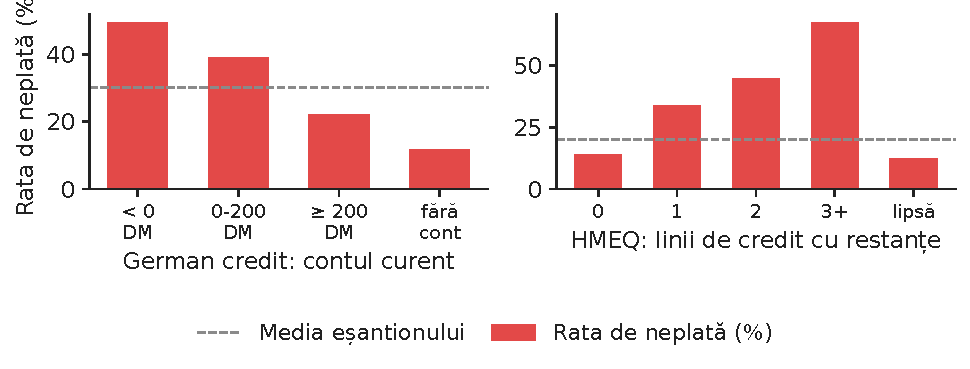
\includegraphics[width=\textwidth,height=0.437\textheight,keepaspectratio]{charts/ro/default_rates.pdf}\end{center}\vspace{-3mm}
\chartsource{Sursa: UCI Statlog German credit; Baesens, Roesch și Scheule (2016), HMEQ. Date: 1\,000 de solicitanți (German credit); 5\,960 de credite (HMEQ).}
\vspace{0.5mm}
\begin{itemize}\setlength{\itemsep}{0pt}
  \item Probabilitatea de neplată (PD): 49{,}3\,\% cu sold negativ în contul curent, 11{,}7\,\% fără cont
    \begin{itemize}\setlength{\itemsep}{0pt}
      \item 14{,}0\,\% fără linii cu restanțe, 67{,}3\,\% cu trei sau mai multe.
    \end{itemize}
\end{itemize}
\par\vfill\manager{un model trebuie să reproducă cel puțin aceste rate pe setul de validare.}\par\vspace{0.5mm}
\par\vfill\noindent{\scriptsize\color{FooterGray}(calcul propriu)}\hfill\qlink{NN\_L1\_default\_rates}{Quantlets/L1/NN_L1_default_rates}\par\vspace{0.5mm}
\end{frame}

\begin{frame}{Învățarea = minimizarea pierderii medii pe datele de antrenare, judecată pe date noi}
\small
\intuition{estimăm pe un eșantion și plătim pentru erorile făcute cu următorii solicitanți.}
\[ \underbrace{\hat R_n(\btheta)=\frac1n\sum_{i=1}^n \ell\big(y_i,f(\vx_i;\btheta)\big)}_{\text{riscul empiric (antrenare)}}\qquad\text{vs.}\qquad \underbrace{R(\btheta)=\E_{(\vx,y)\sim P}\,\ell\big(y,f(\vx;\btheta)\big)}_{\text{riscul pe solicitanți noi}} \]
{\footnotesize\begin{itemize}\setlength{\itemsep}{0pt}
  \item \textbf{\txtwhere}
    \begin{itemize}\setlength{\itemsep}{0pt}
      \item $P$ distribuția necunoscută a viitorilor solicitanți, $\ell$ pierderea, minimizăm $\hat R_n$, banca plătește $R$
    \end{itemize}
\end{itemize}\par}
\begin{itemize}\setlength{\itemsep}{2pt}
  \item Trei seturi: antrenare (estimăm $\btheta$), validare (alegem modelul), testare (raportăm o dată).
  \item HMEQ, stratificat: 3\,576 de credite de antrenare, 1\,192 de validare, 1\,192 de testare.
  \item Fără scurgere de informație: medianele și standardizarea se estimează doar pe partea de antrenare.
\end{itemize}
\par\vfill\manager{setul de testare se folosește o singură dată, la final (schema de validare: cursul 3).}\par\vspace{0.5mm}
\par\vfill\noindent{\scriptsize\color{FooterGray}(Bishop \& Bishop, 2024, ch.~1)}\hfill\tryit{notebook \S2}\par\vspace{0.5mm}
\end{frame}


\section{Modelele liniare sînt rețele cu un singur neuron}

\begin{frame}{Regresia liniară este un neuron fără funcție de activare}
\footnotesize
\intuition{o sumă ponderată a intrărilor plus un termen liber; pierderea pătratică este log-verosimilitatea gaussiană.}
\begin{columns}[T,onlytextwidth]
\begin{column}{0.53\textwidth}
\[ \hat y=\vw^\top\vx+b,\qquad \mathrm{MSE}(\vw,b)=\frac1n\sum_{i=1}^n\big(y_i-\vw^\top\vx_i-b\big)^2 \]
{\footnotesize\begin{itemize}\setlength{\itemsep}{0pt}
  \item \textbf{\txtwhere}
    \begin{itemize}\setlength{\itemsep}{0pt}
      \item $\vx\in\R^d$ intrările, $\vw$ ponderile, $b$ termenul liber
      \item Eroarea pătratică medie (MSE) pierderea
    \end{itemize}
\end{itemize}\par}\[ \varepsilon_i\iid\mathcal N(0,\sigma^2):\ \ -\log L=\tfrac{n}{2}\log 2\pi\sigma^2+\tfrac{n}{2\sigma^2}\mathrm{MSE} \]
\end{column}
\begin{column}{0.44\textwidth}
\begin{itemize}\setlength{\itemsep}{2pt}
  \item Verosimilitate maximă = cele mai mici pătrate: același $\hat\vw=(\mX^\top\mX)^{-1}\mX^\top\vy$.
  \item O rețea nu are o formulă explicită: se antrenează prin coborîre pe gradient (cursul 2).
  \item California, doar latitudinea: MSE în afara eșantionului 0{,}896 pentru dreaptă.
\end{itemize}
\end{column}
\end{columns}
\par\vfill\manager{dreapta de regresie este reperul pe care orice rețea de regresie trebuie să-l depășească în afara eșantionului.}\par\vspace{0.5mm}
\par\vfill\noindent{\scriptsize\color{FooterGray}(Bishop \& Bishop, 2024, ch.~4)}\par\vspace{0.5mm}
\end{frame}

\begin{frame}{Regresia logistică este un neuron cu funcție sigmoidă}
\footnotesize
\intuition{neuronul produce o probabilitate, iar pierderea este minus log-verosimilitatea Bernoulli (entropia încrucișată).}
\begin{columns}[T,onlytextwidth]
\begin{column}{0.53\textwidth}
\[ p_i=\sigma(\vw^\top\vx_i+b)=\frac{1}{1+e^{-z_i}},\qquad \nabla_{\vw}\loss=\frac1n\sum_{i=1}^n (p_i-y_i)\,\vx_i \]
\[ \loss(\vw,b)=-\frac1n\sum_{i=1}^n\big[y_i\log p_i+(1-y_i)\log(1-p_i)\big] \]
{\footnotesize\begin{itemize}\setlength{\itemsep}{0pt}
  \item \textbf{\txtwhere}
    \begin{itemize}\setlength{\itemsep}{0pt}
      \item $z_i$ logitul (logaritmul șansei), $\sigma$ funcția sigmoidă, $y_i\in\{0,1\}$ neplata
      \item Derivarea în anexă
    \end{itemize}
\end{itemize}\par}
\end{column}
\begin{column}{0.44\textwidth}
\begin{itemize}\setlength{\itemsep}{2pt}
  \item Gradientul este eroarea înmulțită cu intrarea: aceeași formă apare în fiecare strat la propagarea înapoi.
  \item $e^{w_j}$ este raportul șanselor pentru o creștere cu o unitate a lui $x_j$.
  \item Pierdere convexă: un singur minim global.
\end{itemize}
\end{column}
\end{columns}
\par\vfill\manager{scorul logistic este standardul industriei pentru modelele PD.}\par\vspace{0.5mm}
\par\vfill\noindent{\scriptsize\color{FooterGray}(Bishop \& Bishop, 2024, ch.~5)}\par\vspace{0.5mm}
\end{frame}

\begin{frame}{Restanțele și lipsa raportului datorii/venit cresc cel mai mult șansa de neplată}
\small
\intuition{HMEQ, intrări standardizate: fiecare coeficient este variația log-șansei la o abatere standard.}
\begin{center}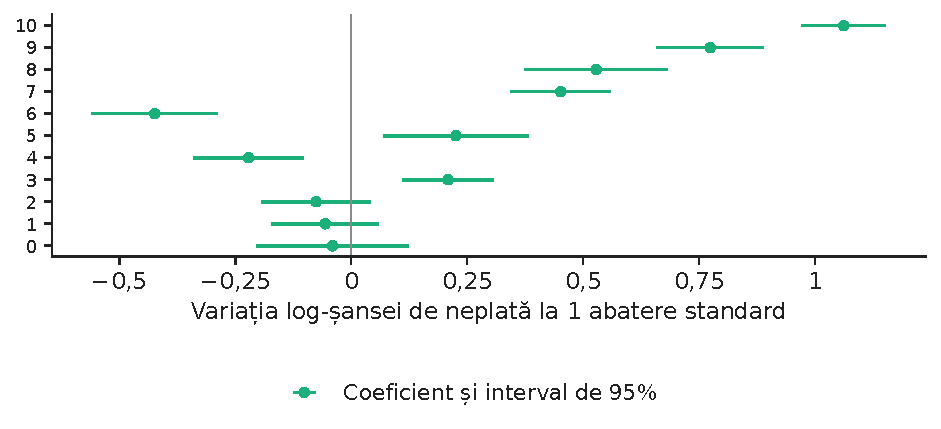
\includegraphics[width=\textwidth,height=0.449\textheight,keepaspectratio]{charts/ro/logit_coef.pdf}\end{center}\vspace{-3mm}
\chartsource{Sursa: Baesens, Roesch și Scheule (2016), datele HMEQ. Date: 3\,576 de credite de antrenare.}
\vspace{0.5mm}
\begin{itemize}\setlength{\itemsep}{0pt}
  \item Rapoartele șanselor $e^{w_j}$: 2{,}89 pentru raportul datorii/venit lipsă, 2{,}17 pentru liniile cu restanțe, 0{,}65 pentru un istoric mai vechi (pseudo-$R^2$ McFadden 0{,}374).
\end{itemize}
\par\vfill\manager{un semn contrar intuiției (valoarea proprietății) este un motiv să analizați datele.}\par\vspace{0.5mm}
\par\vfill\noindent{\scriptsize\color{FooterGray}(calcul propriu)}\hfill\qlink{NN\_L1\_logit\_coef}{Quantlets/L1/NN_L1_logit_coef}\par\vspace{0.5mm}
\end{frame}

\begin{frame}{Propagarea înainte pentru un solicitant real, pas cu pas}
\small
\intuition{scorul este o sumă de contribuții $w_jx_j$; funcția sigmoidă îl transformă într-o probabilitate.}
\begin{columns}[T,onlytextwidth]
\begin{column}{0.50\textwidth}
{\footnotesize\renewcommand{\arraystretch}{1.05}\setlength{\tabcolsep}{4pt}
\begin{tabular}{@{}lrrr@{}}\toprule
Intrare & $x_j$ & $w_j$ & $w_jx_j$ \\ \midrule
linii de credit cu restanțe & 1{,}46 & 0{,}774 & \ensuremath{+}1{,}13 \\
numărul de linii de credit & 2{,}81 & \ensuremath{-}0{,}221 & \ensuremath{-}0{,}62 \\
raport datorii/venit lipsă & \ensuremath{-}0{,}51 & 1{,}062 & \ensuremath{-}0{,}54 \\
termenul liber $b$ &  &  & \ensuremath{-}1{,}99 \\
celelalte 8 intrări &  &  & \ensuremath{+}0{,}31 \\
\textbf{scor $z$} &  &  & \textbf{\ensuremath{-}1{,}71} \\
\bottomrule\end{tabular}}
\end{column}
\begin{column}{0.47\textwidth}
\begin{itemize}\setlength{\itemsep}{2pt}
  \item Solicitant din setul de testare care a intrat ulterior în neplată: credit de 15\,400 USD, raport datorii/venit 36{,}4\,\%, 2 linii cu restanțe.
  \item Ieșirea: $p=\sigma(z)=$ 15{,}3\,\%, sub pragul implicit de 50\,\%.
  \item Intrările $x_j$ sînt standardizate: $x_j=(\text{brut}_j-\bar x_j)/s_j$, cu mediile și abaterile standard de antrenare.
\end{itemize}
\end{column}
\end{columns}
\par\vfill\manager{pragul este o decizie de afaceri: secțiunea 5 îl stabilește din costul unei neplăți neidentificate.}\par\vspace{0.5mm}
\par\vfill\noindent{\scriptsize\color{FooterGray}(calcul propriu)}\hfill\tryit{notebook \S2}\par\vspace{0.5mm}
\end{frame}

\begin{frame}{O valoare lipsă poate fi cel mai puternic semnal}
\small
\intuition{solicitanții care nu își declară raportul datorii/venit intră mult mai des în neplată: lipsa datelor este o informație.}
\[ \tilde x_{ij}=\begin{cases}x_{ij}&\text{observat}\\ \mathrm{med}_{\text{train}}(x_j)&\text{lipsă}\end{cases},\qquad m_{ij}=\mathbb 1\{x_{ij}\ \text{lipsă}\} \]
\begin{itemize}\setlength{\itemsep}{2pt}
  \item Raportul datorii/venit lipsește pentru 21{,}3\,\% dintre creditele HMEQ.
  \item Rata de neplată este 62{,}0\,\% cînd lipsește, față de 8{,}6\,\% cînd este declarat.
  \item Fiecare dintre cele 10 intrări numerice primește o completare cu mediana și un indicator $m_{ij}$
    \begin{itemize}\setlength{\itemsep}{0pt}
      \item Cu 8 variabile binare pentru scop și ocupație, rețeaua vede $d=$ 28 intrări.
    \end{itemize}
\end{itemize}
\par\vfill\manager{nu eliminați rîndurile cu valori lipsă din datele de credit: ați elimina solicitanții cei mai riscanți.}\par\vspace{0.5mm}
\par\vfill\noindent{\scriptsize\color{FooterGray}(Baesens, Rösch \& Scheule, 2016)}\hfill\tryit{notebook \S2}\par\vspace{0.5mm}
\end{frame}


\section{Perceptronul}

\begin{frame}{De la neuronul logic la mașina care învață}
\footnotesize
\intuition{McCulloch și Pitts au scris neuronul ca unitate cu prag; Rosenblatt a făcut ca ponderile lui să învețe din exemple.}
\begin{columns}[T,onlytextwidth]
\begin{column}{0.53\textwidth}
\[ \hat y=\operatorname{step}(\vw^\top\vx+b)=\begin{cases}+1&\vw^\top\vx+b>0\\-1&\text{altfel}\end{cases} \]
{\footnotesize\begin{itemize}\setlength{\itemsep}{0pt}
  \item \textbf{\txtwhere}
    \begin{itemize}\setlength{\itemsep}{0pt}
      \item $\vx$ intrările (dendritele), $\vw$ ponderile sinaptice, $-b$ pragul de activare
      \item $\hat y$ clasa (axonul)
    \end{itemize}
\end{itemize}\par}
\end{column}
\begin{column}{0.44\textwidth}
\begin{itemize}\setlength{\itemsep}{2pt}
  \item 1943: calculul logic al neuronilor cu prag (McCulloch \& Pitts, 1943).
  \item 1958: perceptronul învață $\vw$ din exemple etichetate (Rosenblatt, 1958).
  \item 1969: un singur strat nu poate reprezenta XOR (Minsky \& Papert, 1969).
  \item 1986: propagarea înapoi a erorii antrenează mai multe straturi (Rumelhart, Hinton \& Williams, 1986).
\end{itemize}
\end{column}
\end{columns}
\par\vfill\manager{perceptronul este un clasificator liniar: frontiera lui $\vw^\top\vx+b=0$ este un hiperplan.}\par\vspace{0.5mm}
\par\vfill\noindent{\scriptsize\color{FooterGray}(Bishop \& Bishop, 2024, ch.~5)}\par\vspace{0.5mm}
\end{frame}

\begin{frame}{Perceptronul învață numai din greșelile sale}
\footnotesize
\intuition{cînd un exemplu este clasificat greșit, ponderile se mută spre el; altfel nu se schimbă nimic.}
\begin{columns}[T,onlytextwidth]
\begin{column}{0.53\textwidth}
\[ \text{dacă}\ y_i(\vw^\top\vx_i+b)\le 0:\qquad \vw\leftarrow\vw+\eta\,y_i\vx_i,\quad b\leftarrow b+\eta\,y_i \]
\[ \loss_P(\vw,b)=-\!\!\sum_{i\in\mathcal M}\! y_i(\vw^\top\vx_i+b) \]
{\footnotesize\begin{itemize}\setlength{\itemsep}{0pt}
  \item \textbf{\txtwhere}
    \begin{itemize}\setlength{\itemsep}{0pt}
      \item $y_i\in\{-1,+1\}$, $\eta>0$ rata de învățare, $\mathcal M$ mulțimea exemplelor clasificate greșit
      \item $\loss_P$ criteriul perceptronului
    \end{itemize}
\end{itemize}\par}
\end{column}
\begin{column}{0.44\textwidth}
\begin{itemize}\setlength{\itemsep}{2pt}
  \item Actualizarea este un pas de coborîre stohastică pe gradient (SGD) pe $\loss_P$, pentru un exemplu clasificat greșit.
  \item Spre deosebire de regresia logistică, exemplele corecte nu dau gradient: perceptronul ignoră cît de sigur este.
  \item Nu rezultă nicio probabilitate, ci doar o clasă.
\end{itemize}
\end{column}
\end{columns}
\par\vfill\manager{pentru credit, o clasă fără probabilitate nu poate fi evaluată și nici comparată cu un cost.}\par\vspace{0.5mm}
\par\vfill\noindent{\scriptsize\color{FooterGray}(Rosenblatt, 1958; Bishop \& Bishop, 2024, ch.~5)}\par\vspace{0.5mm}
\end{frame}

\begin{frame}{Dacă clasele pot fi separate, perceptronul se oprește după un număr finit de greșeli}
\small
\intuition{o margine largă între clase înseamnă că sînt necesare puține corecții.}
\[ \exists\,\vw^*,\ \|\vw^*\|=1:\ y_i\,\vw^{*\top}\vx_i\ge\gamma>0\ \ \forall i,\quad \|\vx_i\|\le R\ \ \Longrightarrow\ \ \#\text{greșeli}\le\Big(\frac{R}{\gamma}\Big)^2 \]
{\footnotesize\begin{itemize}\setlength{\itemsep}{0pt}
  \item \textbf{\txtwhere}
    \begin{itemize}\setlength{\itemsep}{0pt}
      \item $\gamma$ marginea celui mai bun hiperplan separator, $R$ raza datelor, termenul liber este inclus în $\vx$ (o constantă 1)
    \end{itemize}
\end{itemize}\par}
\begin{itemize}\setlength{\itemsep}{2pt}
  \item Teorema lui Novikoff (1962): limita nu depinde nici de numărul de exemple, nici de dimensiune.
  \item Ideea demonstrației: $\vw^\top\vw^*$ crește cu cel puțin $\gamma$ la fiecare greșeală, iar $\|\vw\|^2$ cu cel mult $R^2$ (anexa).
  \item Dacă nu există un hiperplan separator, teorema nu spune nimic, iar ponderile se rotesc la nesfîrșit.
\end{itemize}
\par\vfill\manager{datele reale de neplată nu sînt niciodată separabile: solicitanți cu același dosar pot rambursa sau nu.}\par\vspace{0.5mm}
\par\vfill\noindent{\scriptsize\color{FooterGray}(Novikoff, 1962)}\hfill\tryit{notebook \S3}\par\vspace{0.5mm}
\end{frame}

\begin{frame}{Pe credite reale, perceptronul nu se stabilizează niciodată}
\small
\intuition{clasele se suprapun, așa că fiecare epocă corectează unele credite și le strică pe altele.}
\begin{center}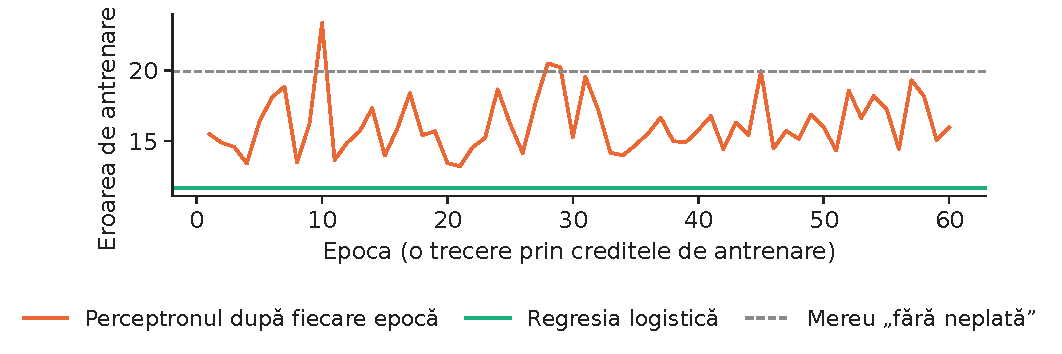
\includegraphics[width=\textwidth,height=0.454\textheight,keepaspectratio]{charts/ro/perceptron_errors.pdf}\end{center}\vspace{-3mm}
\chartsource{Sursa: Baesens, Roesch și Scheule (2016), datele HMEQ. Date: 3\,576 de credite de antrenare.}
\vspace{0.5mm}
\begin{itemize}\setlength{\itemsep}{0pt}
  \item Eroarea după fiecare dintre cele 60 de epoci: 13{,}2--23{,}4\,\%, față de 11{,}7\,\% pentru regresia logistică și 19{,}9\,\% pentru „mereu fără neplată”.
\end{itemize}
\par\vfill\manager{o pierdere netedă și o ieșire probabilistă rezolvă problema: rețelele folosesc sigmoide, nu trepte.}\par\vspace{0.5mm}
\par\vfill\noindent{\scriptsize\color{FooterGray}(calcul propriu)}\hfill\qlink{NN\_L1\_perceptron\_errors}{Quantlets/L1/NN_L1_perceptron_errors}\par\vspace{0.5mm}
\end{frame}

\begin{frame}{Nicio dreaptă nu separă XOR: un strat ascuns reușește}
\small
\intuition{XOR este adevărat cînd exact o intrare este activă; cele două puncte pozitive stau pe o diagonală.}
\vspace{-1mm}\[ h_k=\tanh(\vw_k^\top\vx+b_k),\ k=1,2;\qquad p=\sigma(v_1h_1+v_2h_2+c) \]\vspace{-2mm}
\begin{center}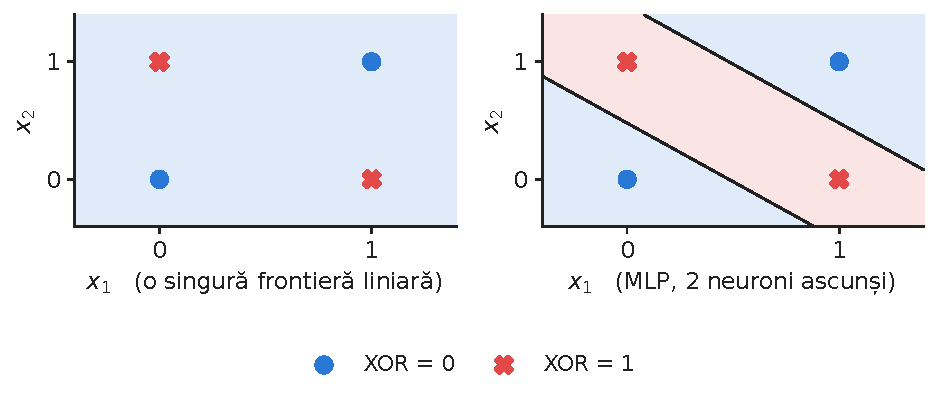
\includegraphics[width=\textwidth,height=0.364\textheight,keepaspectratio]{charts/ro/xor.pdf}\end{center}\vspace{-3mm}
\chartsource{Sursa: tabelul funcției logice XOR (fără date). Date: cele patru intrări XOR.}
\vspace{0.5mm}
\begin{itemize}\setlength{\itemsep}{0pt}
  \item Acuratețea pe cele patru puncte: 50\,\% pentru orice frontieră liniară, 100\,\% cu doi neuroni ascunși.
\end{itemize}
\par\vfill\manager{interacțiunile de tipul „datorii mari și istoric scurt” seamănă cu XOR.}\par\vspace{0.5mm}
\par\vfill\noindent{\scriptsize\color{FooterGray}(Minsky \& Papert, 1969) \simlabel}\hfill\qlink{NN\_L1\_xor}{Quantlets/L1/NN_L1_xor}\par\vspace{0.5mm}
\end{frame}


\section{Perceptronul multistrat}

\begin{frame}{Un MLP alternează transformări afine și activări neliniare}
\small
\intuition{fiecare strat calculează variabile noi din cele anterioare; ultimul strat este o regresie logistică pe ele.}
\[ \vh^{(0)}=\vx,\quad \vh^{(l)}=a\big(\mW^{(l)}\vh^{(l-1)}+\vb^{(l)}\big),\ l=1,\dots,L-1,\quad p(\vx)=\sigma\big(\vw^{(L)\top}\vh^{(L-1)}+b^{(L)}\big) \]
{\footnotesize\begin{itemize}\setlength{\itemsep}{0pt}
  \item \textbf{\txtwhere}
    \begin{itemize}\setlength{\itemsep}{0pt}
      \item $\mW^{(l)}\in\R^{H_l\times H_{l-1}}$, $\vb^{(l)}$ ponderile și termenii liberi ai stratului $l$, de lățime $H_l$ ($H_0=d$), $a$ funcția de activare, element cu element
    \end{itemize}
\end{itemize}\par}
\begin{itemize}\setlength{\itemsep}{2pt}
  \item Fără $a$, straturile se reduc la unul singur: $\mW^{(2)}\mW^{(1)}\vx$ este tot liniar (anexa).
  \item Rețeaua noastră de credit: $d=$ 28 intrări, două straturi ascunse a cîte 64 de unități liniare rectificate (ReLU), o ieșire sigmoidă („MLP 64-64”).
\end{itemize}
\par\vfill\manager{lățimea și adîncimea sînt alegeri de proiectare
    \begin{itemize}\setlength{\itemsep}{0pt}
      \item Secțiunea 5 le alege pe setul de validare.
    \end{itemize}}\par\vspace{0.5mm}
\par\vfill\noindent{\scriptsize\color{FooterGray}(Bishop \& Bishop, 2024, ch.~6)}\hfill\tryit{notebook \S4}\par\vspace{0.5mm}
\end{frame}

\begin{frame}{Funcțiile de activare: netede, ieftine și cu un gradient utilizabil}
\small
\vspace{-1mm}\[ \sigma(z)=\tfrac{1}{1+e^{-z}},\ \ \tanh(z)=\tfrac{e^z-e^{-z}}{e^z+e^{-z}},\ \ \mathrm{ReLU}(z)=\max(0,z),\ \ \mathrm{GELU}(z)=z\,\Phi(z) \]\vspace{-2mm}
\begin{center}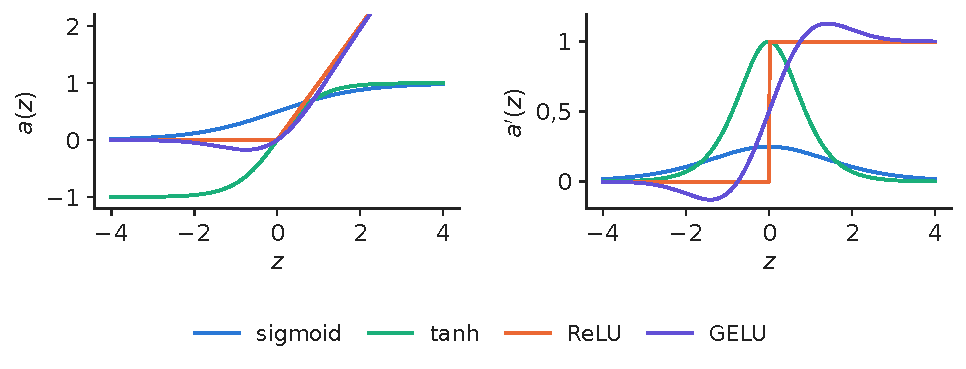
\includegraphics[width=\textwidth,height=0.309\textheight,keepaspectratio]{charts/ro/activations.pdf}\end{center}\vspace{-3mm}
\chartsource{Sursa: funcții analitice (fără date). Date: funcții reprezentate pe [-4, 4].}
\vspace{0.5mm}
\begin{itemize}\setlength{\itemsep}{0pt}
  \item Sigmoida și tanh se saturează ($\sigma'\le$ 0{,}25)
    \begin{itemize}\setlength{\itemsep}{0pt}
      \item Unitatea liniară rectificată (ReLU) transmite gradientul 1 pentru $z>0$
      \item Unitatea liniară cu eroare gaussiană (GELU, $\Phi$ funcția de repartiție normală) apare în arhitecturile transformer.
    \end{itemize}
\end{itemize}
\par\vfill\manager{folosiți ReLU în straturile ascunse
    \begin{itemize}\setlength{\itemsep}{0pt}
      \item Activarea de ieșire decurge din variabila țintă.
    \end{itemize}}\par\vspace{0.5mm}
\par\vfill\noindent{\scriptsize\color{FooterGray}(Bishop \& Bishop, 2024, ch.~6) \simlabel}\hfill\qlink{NN\_L1\_activations}{Quantlets/L1/NN_L1_activations}\par\vspace{0.5mm}
\end{frame}

\begin{frame}{Stratul de ieșire și pierderea decurg din tipul variabilei țintă}
\small
\intuition{fiecare pereche (activare de ieșire, pierdere) este un estimator de verosimilitate maximă pentru o distribuție a lui $y$.}
{\scriptsize\renewcommand{\arraystretch}{1.05}\setlength{\tabcolsep}{4pt}
\begin{tabular}{@{}p{0.20\textwidth}p{0.18\textwidth}p{0.30\textwidth}p{0.24\textwidth}@{}}\toprule
Ținta & Ieșirea & Pierderea & Exemplu \\ \midrule
număr real & $\hat y=z$ & MSE: $\frac1n\sum(y_i-\hat y_i)^2$ & valoarea locuinței, un preț \\
binară & $p=\sigma(z)$ & entropia încrucișată: $-\frac1n\sum[y\log p+(1-y)\log(1-p)]$ & neplată, fraudă \\
$K$ clase & $p_k=\frac{e^{z_k}}{\sum_j e^{z_j}}$ & $-\frac1n\sum_i\log p_{i,y_i}$ & clasa de rating, sentimentul știrilor \\
cuantila $\tau$ & $\hat q=z$ & pinball: $\frac1n\sum\rho_\tau(y_i-\hat q_i)$ & valoarea la risc (VaR), cursul 2 \\
\bottomrule\end{tabular}}
\par\vspace{0.5mm}{\scriptsize \begin{itemize}\setlength{\itemsep}{0pt}
  \item $\rho_\tau(u)=u(\tau-\mathbb 1\{u<0\})$; funcția softmax cu $K=2$ se reduce la sigmoidă.
\end{itemize}}
\par\vfill\manager{un model PD are nevoie de o ieșire sigmoidă și de entropia încrucișată, ca scorurile să fie probabilități.}\par\vspace{0.5mm}
\par\vfill\noindent{\scriptsize\color{FooterGray}(Bishop \& Bishop, 2024, ch.~5--6)}\par\vspace{0.5mm}
\end{frame}

\begin{frame}{Un MLP mic are deja de sute de ori mai mulți parametri decît scorul logistic}
\small
\intuition{fiecare conexiune este o pondere, iar fiecare neuron are un termen liber.}
\[ |\btheta|=\sum_{l=1}^{L}(H_{l-1}+1)\,H_l,\qquad H_0=d,\ H_L=1 \]
\begin{itemize}\setlength{\itemsep}{2pt}
  \item Regresia logistică pe HMEQ: $(d+1)\cdot1=$ 29 de parametri.
  \item MLP 64-64: $(d+1)\cdot64+65\cdot64+65\cdot1=$ 6\,081 de parametri pentru 3\,576 de credite de antrenare.
  \item Mai mulți parametri decît neplăți în datele de antrenare: fără oprire pe baza setului de validare, rețeaua le-ar memora (cursul 3).
  \item Aici fiecare MLP este antrenat cu Adam (cursul 2) și păstrează ponderile din epoca cu cea mai bună pierdere de validare.
\end{itemize}
\par\vfill\manager{numărați parametrii înainte de antrenare: aflați astfel de cîte date și de cîtă regularizare veți avea nevoie.}\par\vspace{0.5mm}
\par\vfill\noindent{\scriptsize\color{FooterGray}}\hfill\tryit{notebook \S4}\par\vspace{0.5mm}
\end{frame}

\begin{frame}{Un singur strat ascuns poate aproxima orice funcție continuă}
\small
\intuition{suficiente „cocoașe” sigmoide, adunate, pot desena orice curbă netedă pe un domeniu mărginit.}
\[ \forall\,g\in C(K),\ \forall\,\varepsilon>0\ \ \exists\,H,\ v_k,\vw_k,b_k:\quad \sup_{\vx\in K}\Big|g(\vx)-\sum_{k=1}^{H}v_k\,\sigma(\vw_k^\top\vx+b_k)\Big|<\varepsilon \]
{\footnotesize\begin{itemize}\setlength{\itemsep}{0pt}
  \item \textbf{\txtwhere}
    \begin{itemize}\setlength{\itemsep}{0pt}
      \item $K\subset\R^d$ compact, $g$ continuă, $\sigma$ sigmoidală (Cybenko, 1989) sau nepolinomială (Hornik, 1991)
    \end{itemize}
\end{itemize}\par}
\begin{itemize}\setlength{\itemsep}{2pt}
  \item Ce spune: familia MLP este suficient de bogată.
  \item Ce nu spune: cît de mare trebuie să fie $H$, dacă coborîrea pe gradient găsește ponderile sau dacă ele generalizează.
\end{itemize}
\par\vfill\manager{teorema justifică încercarea unui MLP
    \begin{itemize}\setlength{\itemsep}{0pt}
      \item Doar testele în afara eșantionului justifică păstrarea lui.
    \end{itemize}}\par\vspace{0.5mm}
\par\vfill\noindent{\scriptsize\color{FooterGray}(Cybenko, 1989; Hornik, 1991)}\par\vspace{0.5mm}
\end{frame}

\begin{frame}{Mai mulți neuroni ascunși urmăresc geografia prețurilor din California}
\small
\intuition{valorile au vîrfuri lîngă Los Angeles și San Francisco; $\hat y(x)=c+\sum_{k=1}^{H}v_k\sigma(w_kx+b_k)$, cu $H=1,3,50$.}
\begin{center}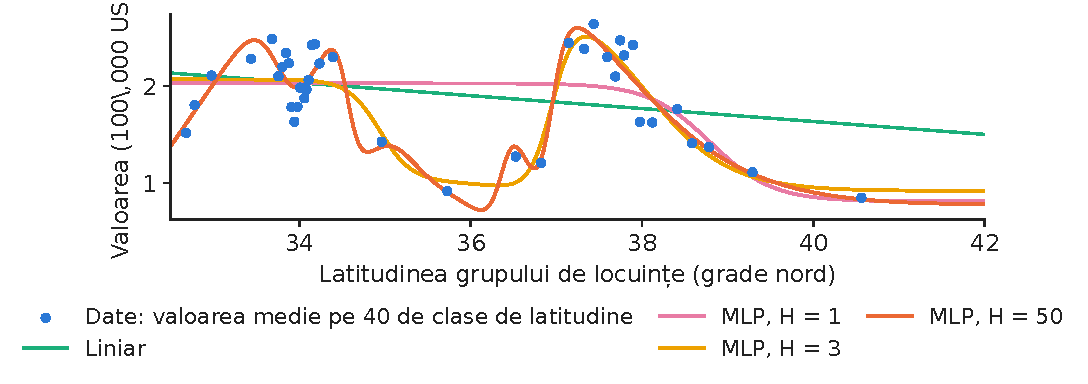
\includegraphics[width=\textwidth,height=0.341\textheight,keepaspectratio]{charts/ro/uat_california.pdf}\end{center}\vspace{-3mm}
\chartsource{Sursa: StatLib, locuințe din California, recensămîntul din 1990 (Pace și Barry, 1997). Date: 19\,648 de grupuri de locuințe sub plafonul sursei.}
\vspace{0.5mm}
\begin{itemize}\setlength{\itemsep}{0pt}
  \item MSE pe datele păstrate deoparte: liniar 0{,}896, $H=1$ 0{,}855, $H=3$ 0{,}757, $H=50$ 0{,}731 (fără cele 992 de grupuri de la plafonul de 500\,000 USD).
\end{itemize}
\par\vfill\manager{efectele de localizare sînt neliniare: un termen liniar în latitudine nu le poate surprinde.}\par\vspace{0.5mm}
\par\vfill\noindent{\scriptsize\color{FooterGray}(calcul propriu)}\hfill\qlink{NN\_L1\_uat\_california}{Quantlets/L1/NN_L1_uat_california}\par\vspace{0.5mm}
\end{frame}

\begin{frame}{Adîncimea refolosește variabilele: o rețea adîncă și îngustă poate întrece una lată}
\small
\intuition{fiecare strat compune variabilele stratului anterior, astfel încît numărul de bucăți liniare poate crește cu adîncimea.}
\[ \text{ReLU MLP:}\ \ f(\vx)\ \text{este liniară pe porțiuni; numărul de regiuni liniare pînă la}\ \ O\big(H^{dL}\big) \]
{\footnotesize\begin{itemize}\setlength{\itemsep}{0pt}
  \item \textbf{\txtwhere}
    \begin{itemize}\setlength{\itemsep}{0pt}
      \item $H$ lățimea fiecărui strat, $L$ numărul de straturi ascunse, $d$ dimensiunea intrării (limita lui Montúfar et al., 2014)
    \end{itemize}
\end{itemize}\par}
\begin{itemize}\setlength{\itemsep}{2pt}
  \item Pentru unele funcții, o rețea puțin adîncă are nevoie de exponențial mai mulți neuroni decît una adîncă.
  \item Pe datele tabelare de credit, două sau trei straturi ascunse sînt de obicei suficiente
    \begin{itemize}\setlength{\itemsep}{0pt}
      \item Adîncimea contează la imagini, text și secvențe.
    \end{itemize}
\end{itemize}
\par\vfill\manager{începeți cu 2 straturi ascunse pe date tabelare
    \begin{itemize}\setlength{\itemsep}{0pt}
      \item Adăugați straturi doar dacă pierderea de validare continuă să scadă.
    \end{itemize}}\par\vspace{0.5mm}
\par\vfill\noindent{\scriptsize\color{FooterGray}(Bishop \& Bishop, 2024, ch.~6)}\par\vspace{0.5mm}
\end{frame}

\begin{frame}{Un MLP curbează frontiera de decizie, dar două intrări aduc puțin semnal în plus}
\small
\intuition{PD prezisă pentru două variabile HMEQ: benzi drepte pentru modelul logistic, regiuni curbe pentru MLP.}
\begin{center}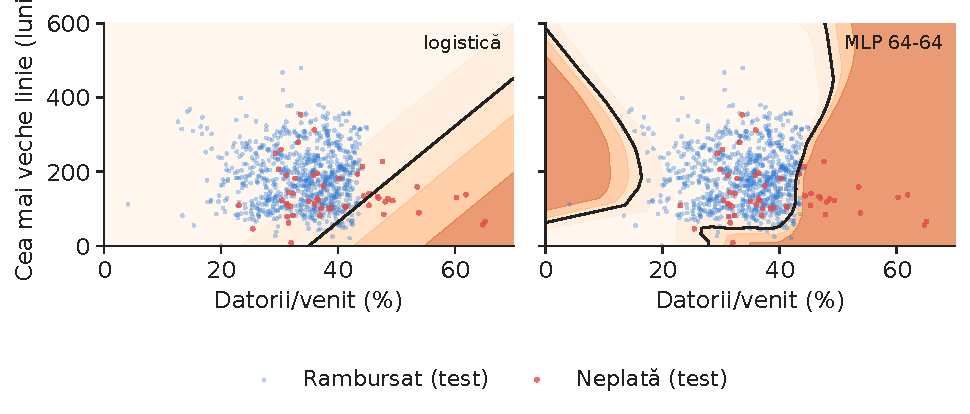
\includegraphics[width=\textwidth,height=0.336\textheight,keepaspectratio]{charts/ro/boundary_hmeq.pdf}\end{center}\vspace{-3mm}
\chartsource{Sursa: Baesens, Roesch și Scheule (2016), datele HMEQ. Date: 2\,708 de credite de antrenare și 871 de testare cu ambele variabile.}
\vspace{0.5mm}
\begin{itemize}\setlength{\itemsep}{0pt}
  \item Aria de sub curbă (AUC) a caracteristicii de operare a receptorului (ROC) = $\Pr(p_{\text{neplată}}>p_{\text{bun}})$
    \begin{itemize}\setlength{\itemsep}{0pt}
      \item Cu aceste două intrări: logistic 0{,}744, MLP 64-64 0{,}736.
    \end{itemize}
\end{itemize}
\par\vfill\manager{o frontieră flexibilă merită doar dacă intrările conțin semnalul.}\par\vspace{0.5mm}
\par\vfill\noindent{\scriptsize\color{FooterGray}(calcul propriu)}\hfill\qlink{NN\_L1\_boundary\_hmeq}{Quantlets/L1/NN_L1_boundary_hmeq}\par\vspace{0.5mm}
\end{frame}


\section{Studiu de caz: scoringul de credit pe credite reale}

\begin{frame}{Protocolul: aceeași împărțire, aceleași intrări, trei modele}
\small
\intuition{o comparație corectă schimbă doar modelul; datele, împărțirea și metrica sînt fixate înainte de orice antrenare.}
\begin{columns}[T,onlytextwidth]
\begin{column}{0.50\textwidth}
\begin{itemize}\setlength{\itemsep}{2pt}
  \item Regresia logistică: verosimilitate maximă, fără penalizare pe HMEQ
    \begin{itemize}\setlength{\itemsep}{0pt}
      \item O penalizare ridge ușoară ($C=1$) pe German credit.
    \end{itemize}
  \item MLP: straturi ReLU, Adam cu rata de învățare $10^{-3}$, loturi de 128 (64 pe German credit), epoca cea mai bună pe validare, 5 inițializări.
  \item Extreme gradient boosting (XGBoost): adîncime 4, rata de învățare 0,03, oprire timpurie pe validare (Chen \& Guestrin, 2016).
\end{itemize}
\end{column}
\begin{column}{0.47\textwidth}
\begin{itemize}\setlength{\itemsep}{2pt}
  \item HMEQ: o împărțire stratificată 60/20/20
    \begin{itemize}\setlength{\itemsep}{0pt}
      \item AUC, curba ROC, calibrarea, intervalul bootstrap al cîștigului de AUC.
    \end{itemize}
  \item German credit: validare încrucișată cu 5 pliuri, repetată de 5 ori (25 de pliuri de test), test $t$ corectat.
  \item Valoarea inițială a generatorului 20261108 (+ indicele rulării)
    \begin{itemize}\setlength{\itemsep}{0pt}
      \item Antrenare pe procesorul central (CPU), sub un minut pe familie de modele.
    \end{itemize}
\end{itemize}
\end{column}
\end{columns}
\par\vfill\manager{scrieți protocolul înainte de antrenare: este primul lucru pe care îl cere cel care validează modelul.}\par\vspace{0.5mm}
\par\vfill\noindent{\scriptsize\color{FooterGray}}\hfill\tryit{notebook \S5}\par\vspace{0.5mm}
\end{frame}

\begin{frame}{Pe HMEQ, un strat ascuns mai lat crește AUC pe test peste scorul logistic}
\small
\intuition{un strat ascuns de lățime $H$; fiecare punct este media a 5 inițializări, banda arată intervalul lor.}
\begin{center}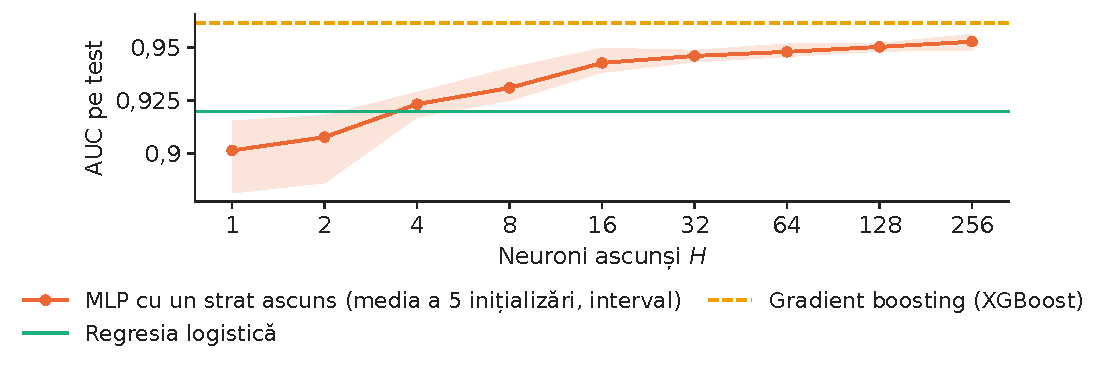
\includegraphics[width=\textwidth,height=0.432\textheight,keepaspectratio]{charts/ro/width_auc.pdf}\end{center}\vspace{-3mm}
\chartsource{Sursa: Baesens, Roesch și Scheule (2016), datele HMEQ. Date: 3\,576 de credite de antrenare\, 1\,192 de validare\, 1\,192 de testare.}
\vspace{0.5mm}
\begin{itemize}\setlength{\itemsep}{0pt}
  \item AUC 0{,}901 la $H=1$, 0{,}953 la $H=$ 256
    \begin{itemize}\setlength{\itemsep}{0pt}
      \item Logistic 0{,}920, XGBoost 0{,}961
      \item Cîștigul se aplatizează după circa 16 neuroni.
    \end{itemize}
\end{itemize}
\par\vfill\manager{aici interacțiunile contează: rețeaua depășește scorul liniar, iar boosting le depășește pe amîndouă.}\par\vspace{0.5mm}
\par\vfill\noindent{\scriptsize\color{FooterGray}(calcul propriu)}\hfill\qlink{NN\_L1\_width\_auc}{Quantlets/L1/NN_L1_width_auc}\par\vspace{0.5mm}
\end{frame}

\begin{frame}{La 10\,\% alarme false, MLP detectează mai multe neplăți decît scorul logistic}
\small
\intuition{curba ROC reprezintă $\Pr(p\ge c\mid\text{neplată})$ în funcție de $\Pr(p\ge c\mid\text{bun})$, pentru fiecare prag $c$.}
\begin{center}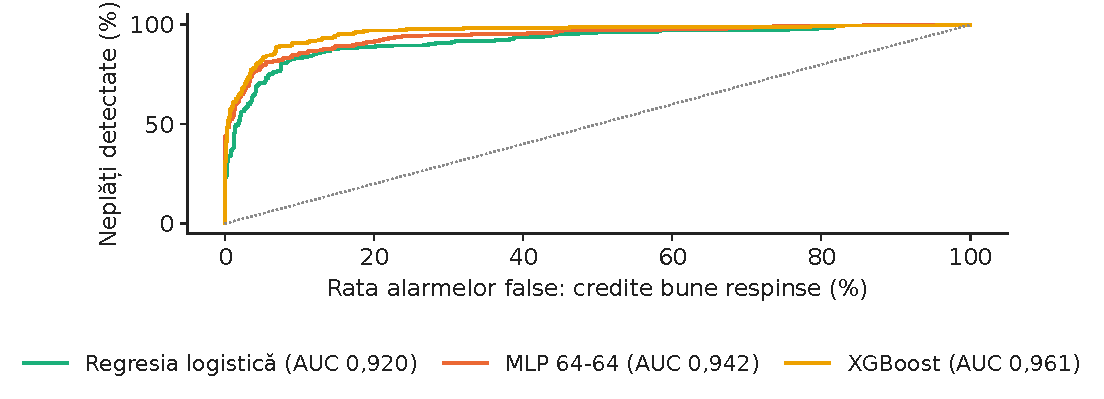
\includegraphics[width=\textwidth,height=0.450\textheight,keepaspectratio]{charts/ro/roc_hmeq.pdf}\end{center}\vspace{-3mm}
\chartsource{Sursa: Baesens, Roesch și Scheule (2016), datele HMEQ. Date: 1\,192 de credite de testare (238 de neplăți).}
\vspace{0.5mm}
\begin{itemize}\setlength{\itemsep}{0pt}
  \item Neplăți detectate cînd respingem 10\,\% dintre creditele bune: logistic 83{,}2\,\%, MLP 85{,}3\,\%, XGBoost 90{,}8\,\% (238 de neplăți în test).
\end{itemize}
\par\vfill\manager{citiți curba la rata de respingere acceptată de afacere, nu doar aria de sub ea.}\par\vspace{0.5mm}
\par\vfill\noindent{\scriptsize\color{FooterGray}(calcul propriu)}\hfill\qlink{NN\_L1\_roc\_hmeq}{Quantlets/L1/NN_L1_roc_hmeq}\par\vspace{0.5mm}
\end{frame}

\begin{frame}{Cîștigul MLP pe HMEQ depășește zgomotul inițializării și al setului de testare}
\small
\intuition{o singură rulare nu dovedește nimic: repetăm antrenarea și reeșantionăm setul de testare.}
\[ \Delta=\mathrm{AUC}_{\mathrm{MLP}}-\mathrm{AUC}_{\text{logit}},\qquad \Delta^{*}_b=\mathrm{AUC}_{\mathrm{MLP}}(\mathcal T^*_b)-\mathrm{AUC}_{\text{logit}}(\mathcal T^*_b),\ b=1,\dots,2000 \]
{\footnotesize\begin{itemize}\setlength{\itemsep}{0pt}
  \item \textbf{\txtwhere}
    \begin{itemize}\setlength{\itemsep}{0pt}
      \item $\mathcal T^*_b$ o reeșantionare bootstrap a celor 1\,192 de credite de testare, aceeași pentru ambele modele (perechi)
    \end{itemize}
\end{itemize}\par}
\begin{itemize}\setlength{\itemsep}{2pt}
  \item Inițializări: MLP 64-64 are în medie AUC pe test 0{,}945 pe 5 inițializări (abaterea standard 0{,}004; interval 0{,}942--0{,}951).
  \item Zgomotul setului de testare: $\Delta=$ 0{,}023, intervalul bootstrap de 95\,\% [0{,}008; 0{,}037]: zero este exclus.
  \item Variația între inițializări a modelului logistic este zero: pierderea lui este convexă.
\end{itemize}
\par\vfill\manager{raportați cîștigul unui model cu un interval
    \begin{itemize}\setlength{\itemsep}{0pt}
      \item Un cîștig mai mic decît variația dintre inițializări nu este un cîștig.
    \end{itemize}}\par\vspace{0.5mm}
\par\vfill\noindent{\scriptsize\color{FooterGray}(calcul propriu)}\hfill\tryit{notebook \S5}\par\vspace{0.5mm}
\end{frame}

\begin{frame}{Scorurile sînt apropiate de probabilități calibrate}
\small
\intuition{în fiecare decilă a PD prezise, rata observată de neplată ar trebui să fie egală cu cea prezisă.}
\begin{center}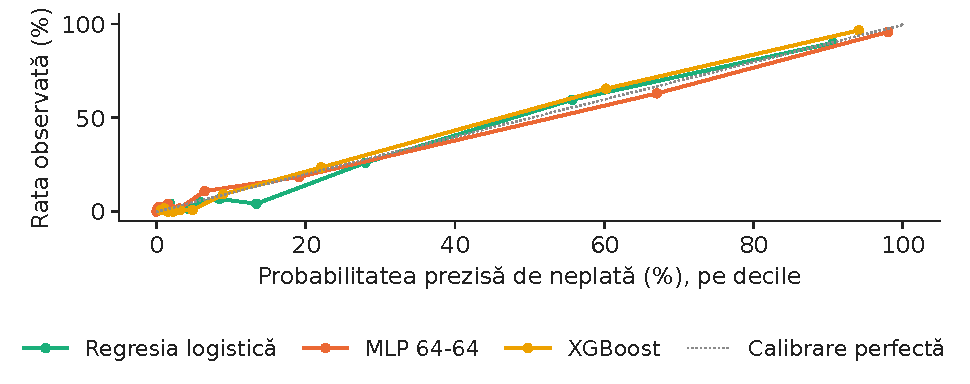
\includegraphics[width=\textwidth,height=0.473\textheight,keepaspectratio]{charts/ro/calibration.pdf}\end{center}\vspace{-3mm}
\chartsource{Sursa: Baesens, Roesch și Scheule (2016), datele HMEQ. Date: 1\,192 de credite de testare.}
\vspace{0.5mm}
\begin{itemize}\setlength{\itemsep}{0pt}
  \item Scorul Brier $\frac1n\sum(p_i-y_i)^2$: logistic 0{,}0742, MLP 0{,}0625, XGBoost 0{,}0549
    \begin{itemize}\setlength{\itemsep}{0pt}
      \item Rata constantă 0{,}1598.
    \end{itemize}
\end{itemize}
\par\vfill\manager{provizioanele și prețurile folosesc PD ca atare: verificați calibrarea, nu doar ordonarea.}\par\vspace{0.5mm}
\par\vfill\noindent{\scriptsize\color{FooterGray}(calcul propriu)}\hfill\qlink{NN\_L1\_calibration}{Quantlets/L1/NN_L1_calibration}\par\vspace{0.5mm}
\end{frame}

\begin{frame}{Pe 1\,000 de solicitanți germani, MLP nu depășește regresia logistică}
\small
\intuition{fiecare punct este AUC pe un pliu de test; bara neagră este media celor 25 de pliuri.}
\begin{center}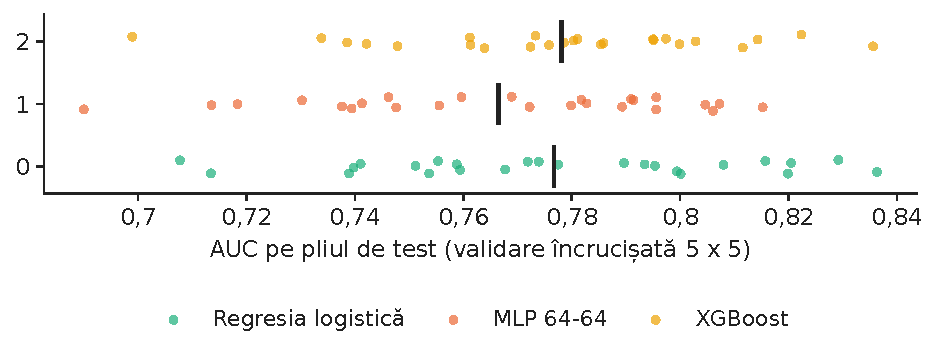
\includegraphics[width=\textwidth,height=0.473\textheight,keepaspectratio]{charts/ro/german_cv.pdf}\end{center}\vspace{-3mm}
\chartsource{Sursa: UCI Machine Learning Repository, Statlog German credit. Date: 1\,000 de solicitanți, 25 de pliuri de test.}
\vspace{0.5mm}
\begin{itemize}\setlength{\itemsep}{0pt}
  \item AUC medie: logistic 0{,}777, MLP 0{,}766, XGBoost 0{,}778
    \begin{itemize}\setlength{\itemsep}{0pt}
      \item MLP minus logistic: $t=$ \ensuremath{-}0{,}93, $p=$ 0{,}362 (slide-ul următor).
    \end{itemize}
\end{itemize}
\par\vfill\manager{cu 1\,000 de rînduri, păstrați scorecard-ul logistic: rețeaua adaugă risc, nu acuratețe.}\par\vspace{0.5mm}
\par\vfill\noindent{\scriptsize\color{FooterGray}(calcul propriu)}\hfill\qlink{NN\_L1\_german\_cv}{Quantlets/L1/NN_L1_german_cv}\par\vspace{0.5mm}
\end{frame}

\begin{frame}{De ce testul $t$ obișnuit exagerează diferențele în validarea încrucișată}
\small
\intuition{seturile de antrenare ale pliurilor diferite se suprapun, deci scorurile pliurilor sînt corelate pozitiv.}
\[ t=\frac{\bar d}{\sqrt{\big(\frac{1}{J}+\frac{n_{\text{test}}}{n_{\text{train}}}\big)\,s_d^2}}\ \sim\ t_{J-1},\qquad d_j=\mathrm{AUC}^{\mathrm{MLP}}_j-\mathrm{AUC}^{\text{logit}}_j \]
{\footnotesize\begin{itemize}\setlength{\itemsep}{0pt}
  \item \textbf{\txtwhere}
    \begin{itemize}\setlength{\itemsep}{0pt}
      \item $J=$ 25 de pliuri, $s_d^2$ varianța de selecție a lui $d_j$, $n_{\text{test}}/n_{\text{train}}=1/4$ pentru 5 pliuri
    \end{itemize}
\end{itemize}\par}
\begin{itemize}\setlength{\itemsep}{2pt}
  \item Termenul $n_{\text{test}}/n_{\text{train}}$ este corecția Nadeau--Bengio: fără ea, $t$ este mult prea mare.
  \item MLP față de logistic: $t=$ \ensuremath{-}0{,}93 ($p=$ 0{,}362)
    \begin{itemize}\setlength{\itemsep}{0pt}
      \item XGBoost față de logistic: $t=$ 0{,}12 ($p=$ 0{,}909).
    \end{itemize}
\end{itemize}
\par\vfill\manager{schimbarea unui model într-o bancă are nevoie de dovezi care rezistă acestei corecții.}\par\vspace{0.5mm}
\par\vfill\noindent{\scriptsize\color{FooterGray}(Nadeau \& Bengio, 2003)}\hfill\tryit{notebook \S6}\par\vspace{0.5mm}
\end{frame}

\begin{frame}{O neplată ratată costă de cinci ori cît un client bun respins: pragul este 1/6, nu 1/2}
\small
\vspace{-1mm}\[ \text{respingem dacă}\ \ c_{\mathrm{FN}}\,p\ \ge\ c_{\mathrm{FP}}(1-p)\iff p\ \ge\ \frac{c_{\mathrm{FP}}}{c_{\mathrm{FP}}+c_{\mathrm{FN}}}=\frac16 \]\vspace{-2mm}
\begin{center}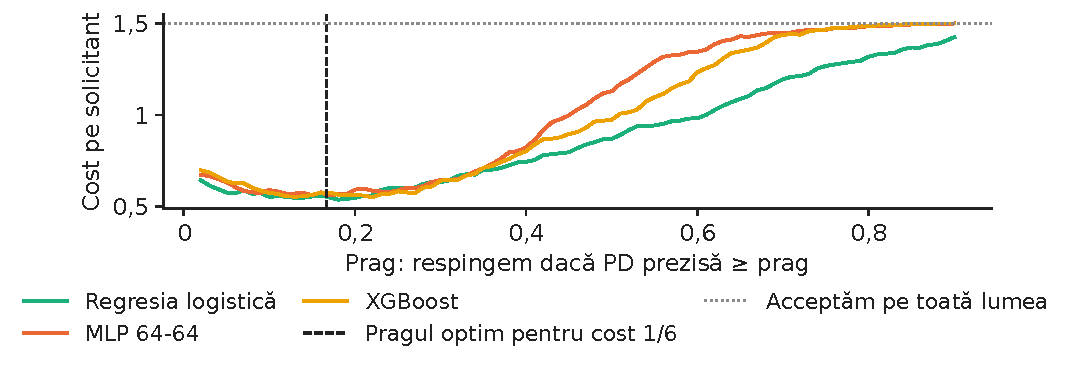
\includegraphics[width=\textwidth,height=0.299\textheight,keepaspectratio]{charts/ro/cost_threshold.pdf}\end{center}\vspace{-3mm}
\chartsource{Sursa: UCI Machine Learning Repository, Statlog German credit. Date: 1\,000 de solicitanți, predicții în afara pliului.}
\vspace{0.5mm}
\begin{itemize}\setlength{\itemsep}{0pt}
  \item Costul pe solicitant (matricea de cost UCI 5:1): la 1/6 logistic 0{,}554, MLP 0{,}568
    \begin{itemize}\setlength{\itemsep}{0pt}
      \item La 1/2 0{,}870 și 1{,}130
      \item Acceptarea tuturor 1{,}50.
    \end{itemize}
\end{itemize}
\par\vfill\manager{aici alegerea pragului contează mai mult decît alegerea modelului.}\par\vspace{0.5mm}
\par\vfill\noindent{\scriptsize\color{FooterGray}(calcul propriu)}\hfill\qlink{NN\_L1\_cost\_threshold}{Quantlets/L1/NN_L1_cost_threshold}\par\vspace{0.5mm}
\end{frame}

\begin{frame}{Un MLP minimal în PyTorch: circa cincisprezece rînduri}
\small
\begin{columns}[T,onlytextwidth]
\begin{column}{0.55\textwidth}
{\ttfamily\scriptsize\setlength{\parindent}{0pt}import torch, torch.nn as nn\\
model = nn.Sequential(\\
~~~~nn.Linear(d, 64), nn.ReLU(),\\
~~~~nn.Linear(64, 64), nn.ReLU(),\\
~~~~nn.Linear(64, 1))~~~~~~~~~~~~\# logit z\\
loss\_fn = nn.BCEWithLogitsLoss()~~\# sigmoid + cross-entropy\\
opt = torch.optim.Adam(model.parameters(), lr=1e-3)\\
for epoch in range(300):\\
~~~~for xb, yb in train\_batches:\\
~~~~~~~~opt.zero\_grad()\\
~~~~~~~~loss = loss\_fn(model(xb), yb)\\
~~~~~~~~loss.backward()~~~~~~~~~~ \# backpropagation\\
~~~~~~~~opt.step()~~~~~~~~~~~~~~~~\# Adam update\\
~~~~\# evaluate on validation, keep the best weights\\
p = torch.sigmoid(model(x\_test))~~ \# predicted PD\par}
\end{column}
\begin{column}{0.42\textwidth}
\begin{itemize}\setlength{\itemsep}{2pt}
  \item \texttt{BCEWithLogitsLoss} combină sigmoida și entropia încrucișată într-o singură funcție, stabilă numeric.
  \item \texttt{backward()} calculează toate gradienții prin propagare înapoi
    \begin{itemize}\setlength{\itemsep}{0pt}
      \item \texttt{step()} aplică optimizatorul: ambele sînt tema cursului 2.
    \end{itemize}
  \item Notebook-ul adaugă pregătirea datelor, oprirea pe baza validării și valorile inițiale ale generatorului.
\end{itemize}
\end{column}
\end{columns}
\par\vfill\manager{aceleași cincisprezece rînduri antrenează toate rețelele tabelare din curs
    \begin{itemize}\setlength{\itemsep}{0pt}
      \item Se schimbă doar datele și straturile.
    \end{itemize}}\par\vspace{0.5mm}
\par\vfill\noindent{\scriptsize\color{FooterGray}(Paszke et al., 2019)}\hfill\tryit{notebook \S7}\par\vspace{0.5mm}
\end{frame}

\begin{frame}{Cînd folosim un MLP pentru date tabelare de afaceri}
\small
\begin{columns}[T,onlytextwidth]
\begin{column}{0.49\textwidth}
\begin{block}{Ce arată acest curs}
\begin{itemize}\setlength{\itemsep}{2pt}
  \item HMEQ, 3\,576 de credite: AUC MLP 0{,}945 față de logistic 0{,}920
    \begin{itemize}\setlength{\itemsep}{0pt}
      \item XGBoost 0{,}961.
    \end{itemize}
  \item German credit, 1\,000 de solicitanți: nicio diferență semnificativă ($p=$ 0{,}362).
  \item În ambele cazuri: pragul din matricea de cost contează mai mult decît modelul.
\end{itemize}
\end{block}
\end{column}
\begin{column}{0.49\textwidth}
\begin{exampleblock}{Regulă practică}
\begin{itemize}\setlength{\itemsep}{2pt}
  \item Puține rînduri, variabile construite, explicație obligatorie: scorecard logistic.
  \item Mii de rînduri, interacțiuni: testați boosting și un MLP față de el.
  \item Text brut, imagini, secvențe, grafuri sau o rețea folosită pentru mai multe sarcini: deep learning.
\end{itemize}
\end{exampleblock}
\end{column}
\end{columns}
\par\vfill\manager{alegeți cel mai simplu model al cărui cîștig în afara eșantionului rezistă la inițializări, reeșantionare și matricea de cost.}\par\vspace{0.5mm}
\end{frame}


\section{Sinteză}

\begin{frame}{Idei principale}
\small
\begin{itemize}\setlength{\itemsep}{4pt}
  \item Regresia liniară și regresia logistică sînt rețele cu un neuron
    \begin{itemize}\setlength{\itemsep}{0pt}
      \item Pierderile lor sînt verosimilități, gradienții lor sînt eroarea înmulțită cu intrarea.
    \end{itemize}
  \item Perceptronul converge doar pe date separabile
    \begin{itemize}\setlength{\itemsep}{0pt}
      \item Datele reale de credit nu sînt separabile, iar XOR arată limita unui singur strat.
    \end{itemize}
  \item Un MLP suprapune transformări afine și activări
    \begin{itemize}\setlength{\itemsep}{0pt}
      \item Un strat ascuns aproximează orice funcție continuă, adîncimea îl face eficient.
    \end{itemize}
  \item Pe credite reale: MLP depășește regresia logistică pe HMEQ (AUC 0{,}945 față de 0{,}920), dar nu pe German credit
    \begin{itemize}\setlength{\itemsep}{0pt}
      \item Boosting este ștacheta.
    \end{itemize}
  \item Evaluați cu mai multe inițializări, intervale, calibrare și costul erorilor, niciodată cu o singură cifră de acuratețe.
\end{itemize}
\end{frame}

\begin{frame}{Ecuațiile principale}
\small
\begin{columns}[T,onlytextwidth]
\begin{column}{0.49\textwidth}
\[ p=\sigma(\vw^\top\vx+b) \]
\[ \loss=-\tfrac1n\textstyle\sum[y\log p+(1-y)\log(1-p)] \]
\[ \nabla_{\vw}\loss=\tfrac1n\textstyle\sum(p_i-y_i)\vx_i \]
\[ \vw\leftarrow\vw+\eta\,y_i\vx_i\ \ \text{dacă e greșit} \]
\end{column}
\begin{column}{0.49\textwidth}
\[ \vh^{(l)}=a\big(\mW^{(l)}\vh^{(l-1)}+\vb^{(l)}\big) \]
\[ |\btheta|=\textstyle\sum_l(H_{l-1}+1)H_l \]
\[ \#\text{greșeli}\le(R/\gamma)^2 \]
\[ \text{respingem dacă}\ p\ge\frac{c_{\mathrm{FP}}}{c_{\mathrm{FP}}+c_{\mathrm{FN}}} \]
\end{column}
\end{columns}
\end{frame}

\begin{frame}{Cercetările grupului nostru: deep learning pentru decizii de afaceri}
\footnotesize
\begin{itemize}\setlength{\itemsep}{2pt}
  \item \textbf{Detectarea explicabilă a fraudei} (Diaconu \& Pele, 2026): a comparat XGBoost și CatBoost cu o rețea neuronală pe grafuri (GNN), eșantionare și agregare pe graf (GraphSAGE), pe datele de fraudă Institute of Electrical and Electronics Engineers, Computational Intelligence Society (IEEE-CIS)
    \begin{itemize}\setlength{\itemsep}{0pt}
      \item Boosting a avut AUC mai mare, modelul pe graf a surprins tiparele relaționale ale fraudei
      \item Un cadru multinivel de inteligență artificială explicabilă (XAI) combină explicațiile aditive Shapley (SHAP) cu eliminarea de noduri și muchii --- replicat în studiul de caz 1 (site-ul cursului).
    \end{itemize}
  \item \textbf{Criptoactivele „zombie”} (Będowska-Sójka, Wójcik \& Pele, 2026): avertizare timpurie, prin învățare automată, pentru criptoactivele care devin „zombie” --- cursul 3.
  \item \textbf{Măsuri de risc obținute din modele lingvistice} (Pele et al., 2026): valoarea la risc (VaR) și pierderea așteptată în coada distribuției (ES), obținute prin interogarea modelelor lingvistice mari (LLM) --- cursul 12.
  \item \textbf{Modele fundație pentru riscul extrem} (Jheng, Tak, Găman, Mazurencu-Marinescu-Pele \& Pele, 2026): VaR și ES fără antrenare (zero-shot), cu calibrare conformală, pe piețele din Europa Centrală și de Est --- cursul 13.
  \item \textbf{Anomaliile pieței văzute ca imagini} (Jheng, Pele, Tak \& Găman, 2026; premiul pentru cea mai bună lucrare la International Conference on Business Excellence (ICBE) 2026): indicatorii pieței, desenați ca imagini, sînt clasificați de un model vizual-lingvistic (VLM), cu justificări în limbaj natural, pe S\&P 500 --- cursul 14.
\end{itemize}
\par\vspace{0.5mm}{\scriptsize \begin{itemize}\setlength{\itemsep}{0pt}
  \item Rezultatele sînt cele declarate în lucrări; cifrele de pe celelalte slide-uri provin din calculele noastre.
\end{itemize}}
\end{frame}

\begin{frame}{Vreți să aflați mai mult?}
\small
\begin{columns}[T,onlytextwidth]
\begin{column}{0.52\textwidth}
\begin{itemize}\setlength{\itemsep}{4pt}
  \item \textbf{Bishop \& Bishop (2024)}, capitolele 4--6: modele liniare, clasificare, rețele adînci: \href{https://www.bishopbook.com}{bishopbook.com}.
  \item \textbf{Dive into Deep Learning}, capitolele 3--5, cu cod PyTorch: \href{https://d2l.ai}{d2l.ai}.
  \item \textbf{Goodfellow, Bengio \& Courville}, capitolul 6: \href{https://www.deeplearningbook.org}{deeplearningbook.org}.
\end{itemize}
\end{column}
\begin{column}{0.45\textwidth}
\begin{itemize}\setlength{\itemsep}{4pt}
  \item \textbf{Tutorialele PyTorch}: \href{https://pytorch.org/tutorials}{pytorch.org/tutorials}.
  \item \textbf{Acest curs}: cod, date, notebook-uri, Quantlets --- \href{https://github.com/danpele/NEURAL_BIZ}{github.com/danpele/NEURAL\_BIZ}.
  \item \textbf{Scoringul de credit în detaliu}: Baesens, Rösch \& Scheule (2016).
\end{itemize}
\end{column}
\end{columns}
\end{frame}

\begin{frame}{Test 1: regresia logistică ca neuron}
\small
\begin{itemize}
  \item Ce pierdere face ca o rețea cu un neuron și ieșire sigmoidă să fie echivalentă cu regresia logistică?
\end{itemize}
\vspace{2mm}
\begin{exampleblock}{R\u{a}spuns}
\begin{itemize}
  \item Entropia încrucișată, adică minus log-verosimilitatea Bernoulli
    \begin{itemize}\setlength{\itemsep}{0pt}
      \item Gradientul ei este $\frac1n\sum(p_i-y_i)\vx_i$.
    \end{itemize}
\end{itemize}
\end{exampleblock}
\end{frame}

\begin{frame}{Test 2: perceptronul pe date reale}
\small
\begin{itemize}
  \item De ce eroarea de antrenare a perceptronului pe HMEQ sare între 13{,}2\,\% și 23{,}4\,\%?
\end{itemize}
\vspace{2mm}
\begin{exampleblock}{R\u{a}spuns}
\begin{itemize}
  \item Clasele nu sînt separabile liniar, deci limita lui Novikoff nu se aplică: fiecare corecție a unui credit le strică pe altele.
\end{itemize}
\end{exampleblock}
\end{frame}

\begin{frame}{Test 3: numărarea parametrilor}
\small
\begin{itemize}
  \item Cîți parametri are un MLP pe intrările HMEQ ($d=$ 28) cu un strat ascuns de 32 de neuroni și o ieșire?
\end{itemize}
\vspace{2mm}
\begin{exampleblock}{R\u{a}spuns}
\begin{itemize}
  \item $(d+1)\cdot32+(32+1)\cdot1=$ 961.
\end{itemize}
\end{exampleblock}
\end{frame}

\begin{frame}{Test 4: pragul optim pentru cost}
\small
\begin{itemize}
  \item O neplată ratată costă 5, un client bun respins costă 1.
    \begin{itemize}\setlength{\itemsep}{0pt}
      \item Peste ce PD ar trebui banca să respingă?
    \end{itemize}
\end{itemize}
\vspace{2mm}
\begin{exampleblock}{R\u{a}spuns}
\begin{itemize}
  \item $p\ge c_{\mathrm{FP}}/(c_{\mathrm{FP}}+c_{\mathrm{FN}})=1/6$
    \begin{itemize}\setlength{\itemsep}{0pt}
      \item Pe German credit, acest prag reduce costul pe solicitant al modelului logistic de la 0{,}870 (pragul 1/2) la 0{,}554.
    \end{itemize}
\end{itemize}
\end{exampleblock}
\end{frame}

\begin{frame}{Test 5: cînd merită un MLP?}
\small
\begin{itemize}
  \item Pe German credit, MLP are AUC medie 0{,}766, iar regresia logistică 0{,}777.
    \begin{itemize}\setlength{\itemsep}{0pt}
      \item Ce recomandați?
    \end{itemize}
\end{itemize}
\vspace{2mm}
\begin{exampleblock}{R\u{a}spuns}
\begin{itemize}
  \item Păstrați scorecard-ul logistic: diferența nu este semnificativă ($p=$ 0{,}362), iar modelul mai simplu este mai ușor de explicat și de validat.
\end{itemize}
\end{exampleblock}
\end{frame}

\begin{frame}{Bibliografie (1/2)}
\scriptsize
\begin{itemize}\setlength{\itemsep}{0pt}\scriptsize
\item Bishop, C.\,M.\ \& Bishop, H.\ (2024). \textit{Deep Learning: Foundations and Concepts}. Springer. \href{https://doi.org/10.1007/978-3-031-45468-4}{doi:10.1007/978-3-031-45468-4}
\item Baesens, B., Rösch, D.\ \& Scheule, H.\ (2016). \textit{Credit Risk Analytics}. Wiley. \href{https://doi.org/10.1002/9781119449560}{doi:10.1002/9781119449560}
\item Będowska-Sójka, B., Wójcik, P.\ \& Pele, D.\,T.\ (2026). Early warning systems for cryptocurrency markets: Predicting `zombie' assets using machine learning. \textit{The North American Journal of Economics and Finance}, 81, 102543. \href{https://doi.org/10.1016/j.najef.2025.102543}{doi:10.1016/j.najef.2025.102543}
\item Chen, T.\ \& Guestrin, C.\ (2016). XGBoost: A scalable tree boosting system. \textit{Proceedings of KDD 2016}, 785--794. \href{https://doi.org/10.1145/2939672.2939785}{doi:10.1145/2939672.2939785}
\item Cybenko, G.\ (1989). Approximation by superpositions of a sigmoidal function. \textit{Mathematics of Control, Signals and Systems}, 2(4), 303--314. \href{https://doi.org/10.1007/BF02551274}{doi:10.1007/BF02551274}
\item Diaconu, D.\ \& Pele, D.\,T.\ (2026). Explainable AI in financial fraud detection: Evidence from the IEEE-CIS fraud dataset. \textit{Proceedings of the International Conference on Business Excellence}, 20(1), 118--132. \href{https://doi.org/10.2478/picbe-2026-0015}{doi:10.2478/picbe-2026-0015}
\item Grinsztajn, L., Oyallon, E.\ \& Varoquaux, G.\ (2022). Why do tree-based models still outperform deep learning on typical tabular data? \textit{Advances in Neural Information Processing Systems}, 35. \href{https://arxiv.org/abs/2207.08815}{arXiv:2207.08815}
\item Hofmann, H.\ (1994). Statlog (German Credit Data). UCI Machine Learning Repository. \href{https://doi.org/10.24432/C5NC77}{doi:10.24432/C5NC77}
\item Hornik, K.\ (1991). Approximation capabilities of multilayer feedforward networks. \textit{Neural Networks}, 4(2), 251--257. \href{https://doi.org/10.1016/0893-6080(91)90009-T}{doi:10.1016/0893-6080(91)90009-T}
\item Jheng, S.-L., Pele, D.\,T., Tak, R.\ \& Găman, Ș.\ (2026). A multimodal vision-language framework for financial anomaly detection. \textit{Proceedings of the International Conference on Business Excellence}, 20(1), 191--201. \href{https://doi.org/10.2478/picbe-2026-0020}{doi:10.2478/picbe-2026-0020}
\item Jheng, S.-L., Tak, R., Găman, Ș., Mazurencu-Marinescu-Pele, M.\ \& Pele, D.\,T.\ (2026). Can foundation models manage risk? Zero-shot VaR and ES forecasting with conformal calibration in CEE markets. \textit{Economic Computation and Economic Cybernetics Studies and Research}, 60(2), 267--290. \href{https://doi.org/10.24818/18423264/60.2.26.14}{doi:10.24818/18423264/60.2.26.14}
\item LeCun, Y., Bengio, Y.\ \& Hinton, G.\ (2015). Deep learning. \textit{Nature}, 521, 436--444. \href{https://doi.org/10.1038/nature14539}{doi:10.1038/nature14539}
\end{itemize}
\end{frame}

\begin{frame}{Bibliografie (2/2)}
\scriptsize
\begin{itemize}\setlength{\itemsep}{0pt}\scriptsize
\item Lessmann, S., Baesens, B., Seow, H.-V.\ \& Thomas, L.\,C.\ (2015). Benchmarking state-of-the-art classification algorithms for credit scoring: An update of research. \textit{European Journal of Operational Research}, 247(1), 124--136. \href{https://doi.org/10.1016/j.ejor.2015.05.030}{doi:10.1016/j.ejor.2015.05.030}
\item McCulloch, W.\,S.\ \& Pitts, W.\ (1943). A logical calculus of the ideas immanent in nervous activity. \textit{The Bulletin of Mathematical Biophysics}, 5(4), 115--133. \href{https://doi.org/10.1007/BF02478259}{doi:10.1007/BF02478259}
\item Minsky, M.\ \& Papert, S.\ (1969). \textit{Perceptrons: An Introduction to Computational Geometry}. MIT Press.
\item Nadeau, C.\ \& Bengio, Y.\ (2003). Inference for the generalization error. \textit{Machine Learning}, 52(3), 239--281. \href{https://doi.org/10.1023/A:1024068626366}{doi:10.1023/A:1024068626366}
\item Novikoff, A.\,B.\,J.\ (1962). On convergence proofs on perceptrons. \textit{Proceedings of the Symposium on the Mathematical Theory of Automata}, 12, 615--622. Polytechnic Institute of Brooklyn.
\item Pace, R.\,K.\ \& Barry, R.\ (1997). Sparse spatial autoregressions. \textit{Statistics \& Probability Letters}, 33(3), 291--297. \href{https://doi.org/10.1016/S0167-7152(96)00140-X}{doi:10.1016/S0167-7152(96)00140-X}
\item Montúfar, G., Pascanu, R., Cho, K.\ \& Bengio, Y.\ (2014). On the number of linear regions of deep neural networks. \textit{Advances in Neural Information Processing Systems}, 27. \href{https://arxiv.org/abs/1402.1869}{arXiv:1402.1869}
\item Paszke, A.\ et al.\ (2019). PyTorch: An imperative style, high-performance deep learning library. \textit{Advances in Neural Information Processing Systems}, 32. \href{https://arxiv.org/abs/1912.01703}{arXiv:1912.01703}
\item Pele, D.\,T., Bolovăneanu, V., Lin, M.-B., Ren, R., Ginavar, A.\,T., Spilak, B., Andrei, A.-V., Toma, F.-M., Lessmann, S.\ \& Härdle, W.\,K.\ (2026). In the beginning was the Word: LLM-VaR and LLM-ES. \textit{Expert Systems with Applications}, 295, 128676. \href{https://doi.org/10.1016/j.eswa.2025.128676}{doi:10.1016/j.eswa.2025.128676}
\item Rosenblatt, F.\ (1958). The perceptron: A probabilistic model for information storage and organization in the brain. \textit{Psychological Review}, 65(6), 386--408. \href{https://doi.org/10.1037/h0042519}{doi:10.1037/h0042519}
\item Rumelhart, D.\,E., Hinton, G.\,E.\ \& Williams, R.\,J.\ (1986). Learning representations by back-propagating errors. \textit{Nature}, 323, 533--536. \href{https://doi.org/10.1038/323533a0}{doi:10.1038/323533a0}
\end{itemize}
\end{frame}

\appendix

\begin{frame}{Anexă: gradientul pierderii logistice}
\small
\[ \sigma'(z)=\sigma(z)\big(1-\sigma(z)\big),\qquad \ell_i=-y_i\log p_i-(1-y_i)\log(1-p_i),\quad p_i=\sigma(z_i) \]
\[ \frac{\partial\ell_i}{\partial z_i}=-\frac{y_i}{p_i}p_i(1-p_i)+\frac{1-y_i}{1-p_i}p_i(1-p_i)=p_i-y_i \]
\[ \frac{\partial\ell_i}{\partial\vw}=\frac{\partial\ell_i}{\partial z_i}\,\frac{\partial z_i}{\partial\vw}=(p_i-y_i)\,\vx_i,\qquad \frac{\partial^2\loss}{\partial\vw\,\partial\vw^\top}=\frac1n\sum_i p_i(1-p_i)\vx_i\vx_i^\top\succeq0 \]
\begin{itemize}\setlength{\itemsep}{2pt}
  \item Hessiana este pozitiv semidefinită: pierderea este convexă, deci coborîrea pe gradient atinge minimul global.
  \item Aceeași regulă de derivare a funcțiilor compuse, aplicată strat cu strat, este propagarea înapoi a erorii (cursul 2).
\end{itemize}
\end{frame}

\begin{frame}{Anexă: demonstrația teoremei de convergență a perceptronului}
\small
\begin{itemize}\setlength{\itemsep}{5pt}
  \item Pornim de la $\vw_0=\mathbf 0$ și notăm cu $\vw_k$ ponderile după a $k$-a greșeală, pe exemplul $(\vx,y)$: $\vw_k=\vw_{k-1}+y\vx$ ($\eta=1$).
  \item Progresul: $\vw_k^\top\vw^*=\vw_{k-1}^\top\vw^*+y\vx^\top\vw^*\ge\vw_{k-1}^\top\vw^*+\gamma$, deci $\vw_k^\top\vw^*\ge k\gamma$.
  \item Creșterea: $\|\vw_k\|^2=\|\vw_{k-1}\|^2+2y\vw_{k-1}^\top\vx+\|\vx\|^2\le\|\vw_{k-1}\|^2+R^2$, pentru că exemplul era greșit
    \begin{itemize}\setlength{\itemsep}{0pt}
      \item Deci $\|\vw_k\|^2\le kR^2$.
    \end{itemize}
  \item Cauchy--Schwarz: $k\gamma\le\vw_k^\top\vw^*\le\|\vw_k\|\le\sqrt k\,R$, de unde $k\le(R/\gamma)^2$.
\end{itemize}
\par\vfill\noindent{\scriptsize\color{FooterGray}(Novikoff, 1962)}\par\vspace{0.5mm}
\end{frame}

\begin{frame}{Anexă: straturile liniare suprapuse se reduc la unul singur}
\small
\[ \mW^{(2)}\big(\mW^{(1)}\vx+\vb^{(1)}\big)+\vb^{(2)}=\underbrace{\mW^{(2)}\mW^{(1)}}_{\mW}\vx+\underbrace{\mW^{(2)}\vb^{(1)}+\vb^{(2)}}_{\vb} \]
\begin{itemize}\setlength{\itemsep}{2pt}
  \item Orice număr de straturi liniare formează o singură transformare liniară: adîncimea fără activare adaugă parametri, nu expresivitate.
  \item Cu o funcție ReLU între ele, $f$ devine liniară pe porțiuni, cu un număr de porțiuni care crește cu adîncimea.
\end{itemize}
\end{frame}

\end{document}
